% https://gateoverflow.in/39667/gate-cse-2016-set-1-question-10#41407

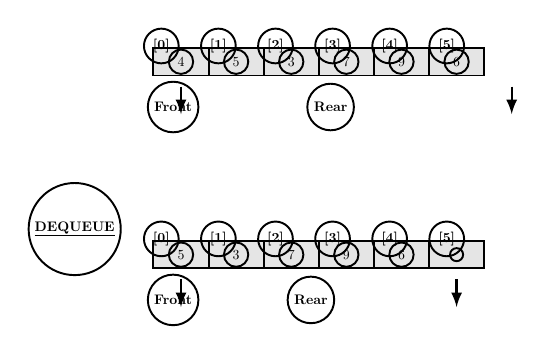
\begin{tikzpicture}[line width=.7pt,scale=0.7]
\begin{scope}
  \draw[fill=gray!20] (0,0)node[xshift=0.2cm,yshift=0.75cm]{$\textbf{[0]}$} rectangle(1,0.5);
  \draw[fill=gray!20] (1,0)node[xshift=0.25cm,yshift=0.75cm]{$\textbf{[1]}$} rectangle(2,0.5);
  \draw[fill=gray!20] (2,0)node[xshift=.3cm,yshift=0.75cm]{$\textbf{[2]}$} rectangle(3,0.5);
  \draw[fill=gray!20] (3,0)node[xshift=0.35cm,yshift=0.75cm]{$\textbf{[3]}$} rectangle(4,0.5);
  \draw[fill=gray!20] (4,0)node[xshift=0.4cm,yshift=0.75cm]{$\textbf{[4]}$} rectangle(5,0.5);
  \draw[fill=gray!20] (5,0)node[xshift=0.45cm,yshift=0.75cm]{$\textbf{[5]}$} rectangle(6,0.5);
  
  \path (0.5,0.25)node{$4$} (1.5,.25)node{$5$} (2.5,.25)node{$3$} (3.5,.25)node{$7$} (4.5,.25)node{$9$} (5.5,.25)node{$6$} ;
  
  %\draw[->,>=latex,thick] (-1.5,0.25) -- (-0.5,0.25);
  %\draw[->,>=latex,thick] (6.5,0.25) -- (7.5,0.25);
  \draw[->,>=latex,thick] (0.5,-0.2) -- (0.5,-0.7);
  \draw[->,>=latex,thick] (6.5,-0.2) -- (6.5,-0.7);
  
  \node[xshift=0.5cm,yshift=-0.8cm]{$\textbf{Front}$};
  \node[xshift=4.5cm,yshift=-0.8cm]{$\textbf{Rear}$};
\end{scope}

\begin{scope}[yshift=-3.5cm]
  \draw[fill=gray!20] (0,0)node[xshift=0.2cm,yshift=0.75cm]{$\textbf{[0]}$} rectangle(1,0.5);
  \draw[fill=gray!20] (1,0)node[xshift=0.25cm,yshift=0.75cm]{$\textbf{[1]}$} rectangle(2,0.5);
  \draw[fill=gray!20] (2,0)node[xshift=.30cm,yshift=0.75cm]{$\textbf{[2]}$} rectangle(3,0.5);
  \draw[fill=gray!20] (3,0)node[xshift=0.35cm,yshift=0.75cm]{$\textbf{[3]}$} rectangle(4,0.5);
  \draw[fill=gray!20] (4,0)node[xshift=0.40cm,yshift=0.75cm]{$\textbf{[4]}$} rectangle(5,0.5);
  \draw[fill=gray!20] (5,0)node[xshift=0.45cm,yshift=0.75cm]{$\textbf{[5]}$} rectangle(6,0.5);
  
  \path (0.5,0.25)node{5} (1.5,.25)node{$3$} (2.5,.25)node{$7$} (3.5,.25)node{$9$} (4.5,.25)node{$6$} (5.5,.25)node{} ;
  
 % \draw[->,>=latex,thick] (-1.5,0.25) -- (-0.5,0.25);
 % \draw[->,>=latex,thick] (6.5,0.25) -- (7.5,0.25);
  \draw[->,>=latex,thick] (0.5,-0.2) -- (0.5,-0.7);
  \draw[->,>=latex,thick] (5.5,-0.2) -- (5.5,-0.7);
  
  \node[xshift=0.5cm,yshift=-0.8cm]{$\textbf{Front}$};
  \node[xshift=4cm,yshift=-0.8cm]{$\textbf{Rear}$};
  \node[xshift=-2cm,yshift=1cm]{$\underline{\textbf{DEQUEUE}}$};
\end{scope}
\end{tikzpicture}

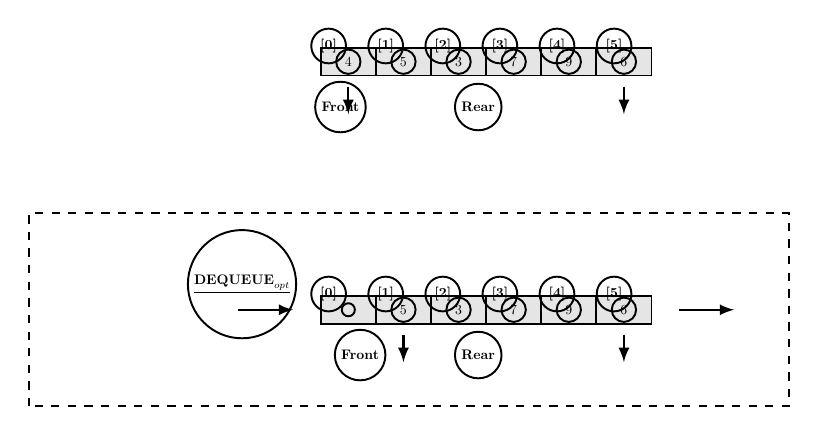
\begin{tikzpicture}[line width=.7pt,scale=0.7]
\begin{scope}
  \draw[fill=gray!20] (0,0)node[xshift=0.2cm,yshift=0.75cm]{$\textbf{[0]}$} rectangle(1,0.5);
  \draw[fill=gray!20] (1,0)node[xshift=0.25cm,yshift=0.75cm]{$\textbf{[1]}$} rectangle(2,0.5);
  \draw[fill=gray!20] (2,0)node[xshift=.3cm,yshift=0.75cm]{$\textbf{[2]}$} rectangle(3,0.5);
  \draw[fill=gray!20] (3,0)node[xshift=0.35cm,yshift=0.75cm]{$\textbf{[3]}$} rectangle(4,0.5);
  \draw[fill=gray!20] (4,0)node[xshift=0.4cm,yshift=0.75cm]{$\textbf{[4]}$} rectangle(5,0.5);
  \draw[fill=gray!20] (5,0)node[xshift=0.45cm,yshift=0.75cm]{$\textbf{[5]}$} rectangle(6,0.5);
  
  \path (0.5,0.25)node{$4$} (1.5,.25)node{$5$} (2.5,.25)node{$3$} (3.5,.25)node{$7$} (4.5,.25)node{$9$} (5.5,.25)node{$6$} ;
  
  %\draw[->,>=latex,thick] (-1.5,0.25) -- (-0.5,0.25);
  %\draw[->,>=latex,thick] (6.5,0.25) -- (7.5,0.25);
  \draw[->,>=latex,thick] (0.5,-0.2) -- (0.5,-0.7);
  \draw[->,>=latex,thick] (5.5,-0.2) -- (5.5,-0.7);
  
  \node[xshift=0.5cm,yshift=-0.8cm]{$\textbf{Front}$};
  \node[xshift=4cm,yshift=-0.8cm]{$\textbf{Rear}$};
\end{scope}

\begin{scope}[yshift=-4.5cm]
  \draw[fill=gray!20] (0,0)node[xshift=0.20cm,yshift=0.75cm]{$\textbf{[0]}$} rectangle(1,0.5);
  \draw[fill=gray!20] (1,0)node[xshift=0.25cm,yshift=0.75cm]{$\textbf{[1]}$} rectangle(2,0.5);
  \draw[fill=gray!20] (2,0)node[xshift=.30cm,yshift=0.75cm]{$\textbf{[2]}$} rectangle(3,0.5);
  \draw[fill=gray!20] (3,0)node[xshift=0.35cm,yshift=0.75cm]{$\textbf{[3]}$} rectangle(4,0.5);
  \draw[fill=gray!20] (4,0)node[xshift=0.40cm,yshift=0.75cm]{$\textbf{[4]}$} rectangle(5,0.5);
  \draw[fill=gray!20] (5,0)node[xshift=0.45cm,yshift=0.75cm]{$\textbf{[5]}$} rectangle(6,0.5);
  
  \path (0.5,0.25)node{${}$} (1.5,.25)node{$5$} (2.5,.25)node{$3$} (3.5,.25)node{$7$} (4.5,.25)node{$9$} (5.5,.25)node{$6$} ;
  
  \draw[->,>=latex,thick] (-1.5,0.25) -- (-0.5,0.25);
  \draw[->,>=latex,thick] (6.5,0.25) --  (7.5,0.25);
  \draw[->,>=latex,thick] (1.5,-0.2) --  (1.5,-0.7);
  \draw[->,>=latex,thick] (5.5,-0.2) --  (5.5,-0.7);
  
  \node[xshift=4cm,yshift=-0.8cm]{$\textbf{Rear}$};
  \node[xshift=1cm,yshift=-0.8cm]{$\textbf{Front}$};
  \node[xshift=-2cm,yshift=1cm]{$\underline{\textbf{DEQUEUE}_{\text{opt}}} $};
  
  \draw[dashed](-5.3,-1.5) rectangle (8.5,2);
  
  
  
\end{scope}
  
\end{tikzpicture}

%https://gateoverflow.in/39716/gate-cse-2016-set-1-question-48?show=40194#a40194
 \tikzset{
    rubberduck/.style={
        draw=black!90,
        fill = white,
        shape=isosceles triangle,
        minimum height=5.5cm,
        minimum width=2cm,
        shape border rotate=#1,
        isosceles triangle stretches,
        inner sep=0pt,ultra thick
    },
    rubber/.style={rubberduck=+120},
    ducky/.style={rubberduck=-90}}
 
 
 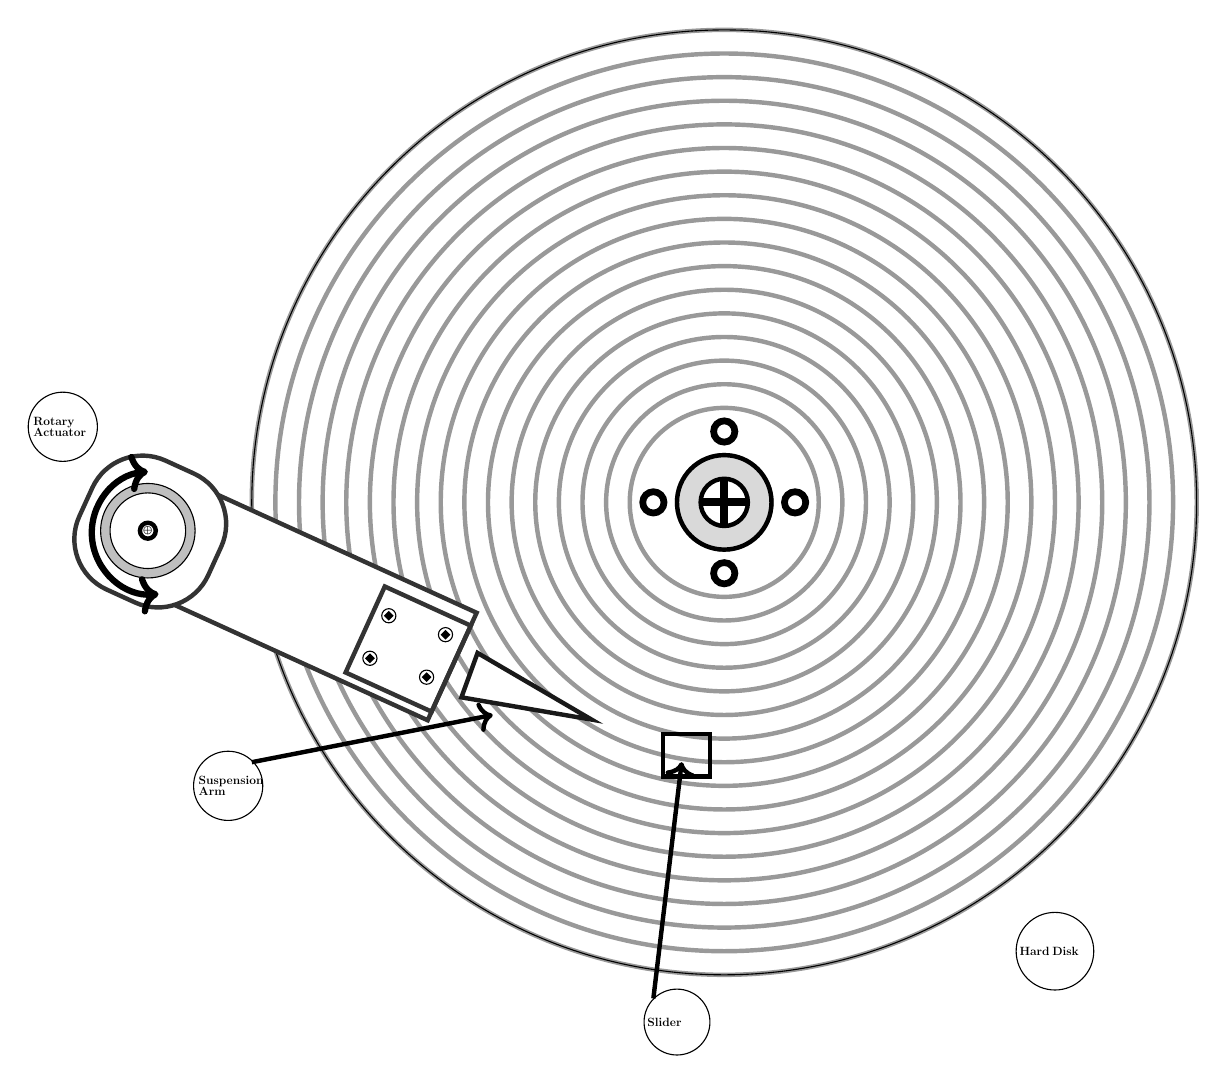
\begin{tikzpicture}[scale=0.6,transform shape]
      \foreach \x in {10,20,25,30,35,40,45,50,55,60,65,70,75,80,85,90,95,100}
        \pgfmathsetmacro{\tmp}{0.1*\x}
        \draw[color=black!40,ultra thick] (0,0) circle (\tmp cm); 
        \draw (0,0) node[circle,inner sep=1.5pt,fill,ultra thick] {} circle [radius=10];
        
 
    
 \node[draw,circle,minimum size=4cm,ultra thick,fill = gray!30] at (0,0){};
 \node[draw,circle,minimum size=2cm,ultra thick,fill=white] at (0,0){};
       
       
 \draw[-,line width = 1mm](0,0.5) -- (0,-.5);
           \draw[-,line width = 1mm](0.5,0) -- (-0.5,0);
           
\node[draw,circle,minimum size=1cm,ultra thick] at (-1.5,0){};
\node[draw,circle,minimum size=0.8cm,ultra thick] at (-1.5,0){};
            
\node[draw,circle,minimum size=1cm,ultra thick] at (1.5,0){};
\node[draw,circle,minimum size=0.8cm,ultra thick] at (1.5,0){};
            
 \node[draw,circle,minimum size=1cm,ultra thick] at (0,1.5){};
\node[draw,circle,minimum size=0.8cm,ultra thick] at (0,1.5){};
            
\node[draw,circle,minimum size=1cm,ultra thick] at (0,-1.5){};
\node[draw,circle,minimum size=0.8cm,ultra thick] at (0,-1.5){};
     
\draw[draw=black,ultra thick] (-1.3,-5.8) rectangle ++(1,0.9);

%R2
\draw[draw=black,ultra thick,color = black!80,rotate=-24.5,fill = white] (-9.8,-6.8) rectangle ++(6,2.5);
%R1
\draw[draw=black,ultra thick,color = black!80,rotate=-24.5] (-5.8,-6.6) rectangle ++(2,2);
%rr
\draw[draw=black,ultra thick,color = black!80,rotate=-24.5,rounded corners=20pt,fill=white] (-12.3,-7.1)  rectangle ++(3,3);

     \draw (-6.3,-3.7) node[circle,inner sep=1.5pt,fill,ultra thick] {} circle [radius=0.15];
      \draw (-5.9,-2.8) node[circle,inner sep=1.5pt,fill,ultra thick] {} circle [radius=0.15];
    
\draw (-7.5,-3.3) node[circle,inner sep=1.5pt,fill,ultra thick] {} circle [radius=0.15];
      \draw (-7.1,-2.4) node[circle,inner sep=1.5pt,fill,ultra thick] {} circle [radius=0.15];
        \node[rubber,rotate=-110] at (-5,-3.8){};
   %%%anular   
   \draw[fill=gray!50] (-12.2,-0.6) node[circle,inner sep=1.5pt,fill,ultra thick,] {} circle [radius=1];
\draw[fill=white] (-12.2,-0.6) node[circle,inner sep=1.5pt,ultra thick] {$\bigoplus$} circle [radius=0.8];

\node[text width=2.5cm] at (-14,1.6) {\textbf{\Large{Rotary Actuator}}};
\node[text width=3cm] at (7,-9.5) {\textbf{\Large{Hard Disk}}};

\node[text width=2.5cm] at (-10.5,-6) {\textbf{\Large{Suspension Arm}}};

\node[text width=2.5cm] at (-1,-11) {\textbf{\Large{Slider}}};

\draw[->,ultra thick] (-1.5,-10.5) -- (-0.9,-5.5);
\draw[->,ultra thick] (-10,-5.5) -- (-4.9,-4.5);


 \path [draw=black,rotate=90,<->, ultra thick,line width = 0.8mm ] (0.65,12.2) arc (5:185:1.3cm);
   

      
  \end{tikzpicture}




% https://gateoverflow.in/39669/gate-cse-2016-set-1-question-11


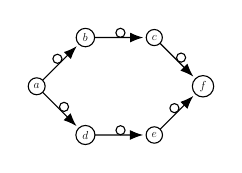
\begin{tikzpicture}[shorten >=1pt,node distance=2.5cm,on grid,auto,scale=0.7,transform shape,font=\large]


    \node[state] (q_0)  {$a$};
    \node[state] (q_1) [above right of=q_0]  {$b$};
    \node[state] (q_2) [right of=q_1] {$c$};
    \node[state] (q_3) [below right of=q_0] {$d$};
    \node[state] (q_4) [right of=q_3] {$e$};
    \node[state] (q_5) [below right of=q_2] {$f$};

     \path[->,-Latex]
       
        (q_0) edge node {} (q_1)
              edge node {} (q_3)
        (q_1) edge node {} (q_2)
        (q_2) edge node {} (q_5)
        (q_3) edge node {} (q_4)
        (q_4) edge node {} (q_5) ;
             
\end{tikzpicture}

%https://gateoverflow.in/39592/gate-cse-2016-set-2-question-50
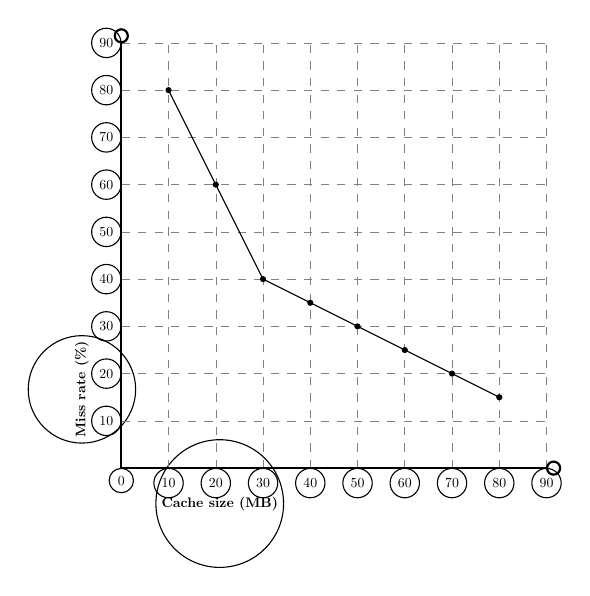
\begin{tikzpicture}[scale = 0.6]
\node[ xshift=2.5cm,yshift=-0.9cm,font=\color{black}] {\textbf{Cache size (MB)}};
  \node[rotate=90,xshift=2cm,yshift=1cm,font=\color{black}] {\textbf{Miss rate (\%)}};
\draw[help lines, color=black!50, dashed] (0,0) grid (9,9);
\draw[thick] (0,0)--(9,0) node[right]{};
\draw[thick] (0,0)--(0,9) node[above]{};
\draw[black] (1,8) -- (2,6) -- (3,4);
\draw[black] (3,4) -- (4,3.5) -- (5,3) -- (6,2.5) -- (7,2) -- (8,1.5);
\filldraw (1,8) circle (1.5pt);
\filldraw (2,6) circle (1.5pt);
\filldraw (3,4) circle (1.5pt);
\filldraw (4,3.5) circle (1.5pt);
\filldraw (5,3) circle (1.5pt);
\filldraw (6,2.5) circle (1.5pt);
\filldraw (7,2) circle (1.5pt);
\filldraw (8,1.5) circle (1.5pt);
\node[below] at (0,0) {$0$};
\node[below] at (1,0) {$10$};
\node[below] at (2,0) {$20$};
\node[below] at (3,0) {$30$};
\node[below] at (4,0) {$40$};
\node[below] at (5,0) {$50$};
\node[below] at (6,0) {$60$};
\node[below] at (7,0) {$70$};
\node[below] at (8,0) {$80$};
\node[below] at (9,0) {$90$};

\node[left] at (0,1) {$10$};
\node[left] at (0,2) {$20$};
\node[left] at (0,3) {$30$};
\node[left] at (0,4) {$40$};
\node[left] at (0,5) {$50$};
\node[left] at (0,6) {$60$};
\node[left] at (0,7) {$70$};
\node[left] at (0,8) {$80$};
\node[left] at (0,9) {$90$};

\end{tikzpicture}

% https://gateoverflow.in/39585/gate-cse-2016-set-2-question-34?show=40018

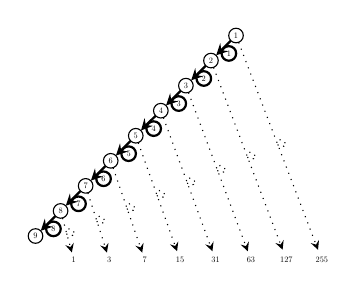
\begin{tikzpicture}[scale=0.6,transform shape,node distance = 1.5cm,on grid,auto,
    every state/.style = {draw = black, fill = white},every initial by arrow/.style = {font = \Large,text = black,
        thick,-stealth}]

 \node[state] (q_0)  {$1$};
 \node[state] (q_1)  [below left of=q_0]  {$2$};
 \node[state] (q_2)  [below left of=q_1]  {$3$};
 \node[state] (q_3)  [below left of=q_2]  {$4$};
 \node[state] (q_4)  [below left of=q_3]  {$5$};
 \node[state] (q_5)  [below left of=q_4]  {$6$};
 \node[state] (q_6)  [below left of=q_5]  {$7$};
 \node[state] (q_7)  [below left of=q_6]  {$8$};
 \node[state] (q_8)  [below left of=q_7]  {$9$};
 \node[state,style={draw=white}] (q_9)  [below right of=q_7,xshift=-0.5cm,yshift=-1cm]  {1};
  \node[state,style={draw=white}] (q_9a)  [right of=q_9]  {3};
 \node[state,style={draw=white}] (q_10)  [right of=q_9a]  {$7$};
 \node[state,style={draw=white}] (q_11)  [right of=q_10]  {$15$};
 \node[state,style={draw=white}] (q_12)  [right of=q_11]  {$31$};
 \node[state,style={draw=white}] (q_13)  [right of=q_12]  {$63$};
 \node[state,style={draw=white}] (q_14)  [right of=q_13]  {$127$};
 \node[state,style={draw=white}] (q_15)  [right of=q_14]  {$255$};
 
 
 \path [-stealth, thick]
 
 (q_0) edge node {1} (q_1)
 (q_1) edge node {2} (q_2)
 (q_2) edge node {3} (q_3)
 (q_3) edge node {4} (q_4)
 (q_4) edge node {5} (q_5)
 (q_5) edge node {6} (q_6)
 (q_6) edge node {7} (q_7)
 (q_7) edge node {8} (q_8);
  \path [-stealth, dotted]
   (q_7)    edge node {} (q_9)
 (q_6) edge node {} (q_9a)
 (q_5) edge node {} (q_10)
 (q_4) edge node {} (q_11)
 (q_3) edge node {} (q_12)
 (q_2) edge node {} (q_13)
 (q_1) edge node {} (q_14)
 (q_0) edge node {} (q_15);
 
\end{tikzpicture}



%https://gateoverflow.in/108484/gate2016-aptitude-set-3-ga-6
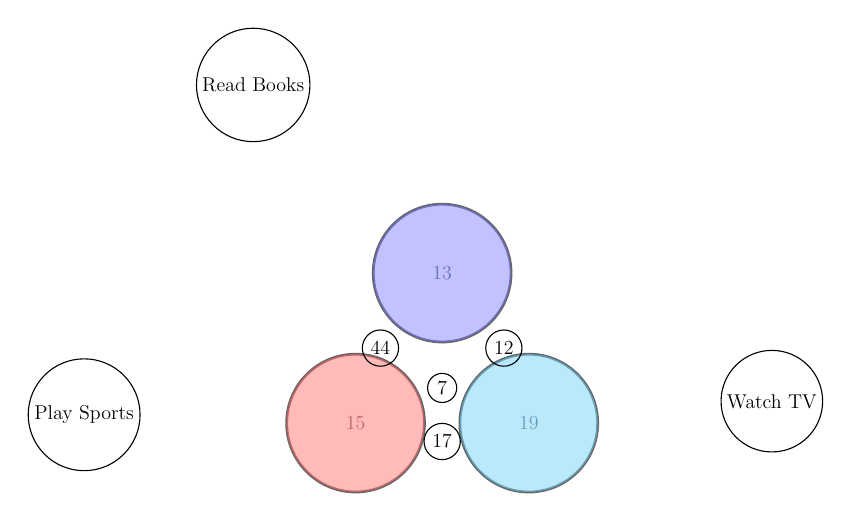
\begin{tikzpicture}[scale=1]
  \tikzset{venn circle/.style={draw,circle,minimum width=3.5cm,fill=#1,opacity=0.6}}
   \begin{scope}[blend group = soft light]

  \node [venn circle = red!45!white,font=\Large] (A) at (0,0) {$15$};
  \node [venn circle = blue!40!white,font=\Large] (B) at (60:2.2cm) {$13$};
  \node [venn circle = cyan!45!white,font=\Large] (C) at (0:2.2cm) {$19$};
  \end{scope}
  \node[left,font=\Large] at (barycentric cs:A=1/2,B=1/2 ) {$44$}; 
  \node[below,font=\Large] at (barycentric cs:A=1/2,C=1/2 ) {$17$};   
  \node[right,font=\Large] at (barycentric cs:B=1/2,C=1/2 ) {$12$};   
  \node[below,font=\Large] at (barycentric cs:A=1/3,B=1/3,C=1/3 ){7};
  \node[above] at (110:3.8cm) {\Large{Read Books}};
  \node[above] at (-4:5.3cm) {\Large{Watch TV}};
  \node[above] at (10:-3.5cm) {\Large{Play Sports}};
  
\end{tikzpicture}  



%https://gateoverflow.in/39727/gate2016-1-40?show=69673#a69673
% diagram G
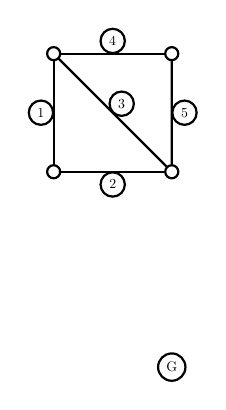
\begin{tikzpicture}[thick,node distance = 3cm,auto,scale = 0.1]
\node[state](1){};
\node[state](2)[right of = 1]{};
\node[state](3)[below of = 1]{};
\node[state](4)[below of = 2]{};

\path (1) edge node{$4$} (2);
\path (1) edge[left] node {$1$} (3);
\path (1) edge node {$3$} (4);
\path (2) edge node {$5$} (4);
\path (3) edge[below] node{$2$} (4);
\node[below] at (15,-38){G} ;

\end{tikzpicture}


%https://gateoverflow.in/39727/gate2016-1-40?show=69673#a69673
% diagram MST
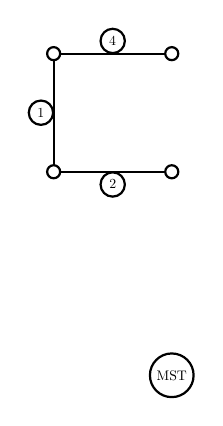
\begin{tikzpicture}[thick,node distance = 3cm,auto,scale = 0.1]
\node[state](1){};
\node[state](2)[right of = 1]{};
\node[state](3)[below of = 1]{};
\node[state](4)[below of = 2]{};

\path (1) edge node{$4$} (2);
\path (1) edge[left] node {$1$} (3);
\path (3) edge[below] node{$2$} (4);
\node[below] at (15,-38){MST} ;

\end{tikzpicture}

%https://gateoverflow.in/39731/gate-cse-2016-set-1-question-38#44143
%https://gateoverflow.in/39731/gate2016-1-38?show=44143#a44143
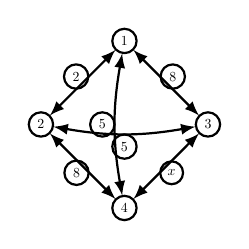
\begin{tikzpicture}[<->,>=latex,,thick,node distance = 3cm,auto,scale = 0.1]
\node[state](1){$1$};
\node[state](2)[below left of = 1]{$2$};
\node[state](3)[below right of = 1]{$3$};
\node[state](4)[below right of = 2]{$4$};

\path (1) edge[above,pos = 0.6] node{$2$} (2);
\path (1) edge[above,pos = 0.6] node{$8$} (3);
\path (2) edge[left,pos = 0.6] node{$8$} (4);
\path (4) edge[right,pos = 0.4] node{$x$} (3);
\path (1) edge[left=30,pos = 0.5,bend right=10] node{$5$} (4);
\path (2) edge[below=30,pos = 0.5,bend right=10] node{$5$} (3);

\end{tikzpicture}



%%%%%%%%https://gateoverflow.in/39581/gate2016-2-39

\usetikzlibrary{shapes,arrows}

% Define block styles
\tikzstyle{decision} = [diamond, draw,  
    text width=4.5em, text badly centered, node distance=3cm, inner sep=3pt]
\tikzstyle{block} = [rectangle, draw,  
    text width=7em, text centered, minimum height=2em,inner sep=4pt]
\tikzstyle{line} = [draw, -latex']
\tikzstyle{cloud} = [draw, rounded rectangle, node distance=3cm,
    minimum height=2em,inner sep=4pt]
    
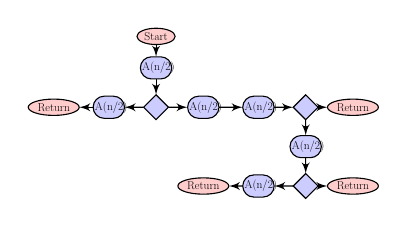
\begin{tikzpicture}[node distance = 2cm, auto,transform shape,scale=0.4,font=\huge]
    % Place nodes
   
    \node [cloud,] (init) {Start};
    \node [block, below of=init] (1) { A(n/2)};
   
    \node [decision, below of=1,node distance = 2.5cm] (decide) {};
     \node [block, left of=decide, node distance=3cm] (2) {A(n/2)};
       \node [cloud,left of = 2,node distance=3.5cm] (return1) {Return};
    \node [block, right of = decide, node distance=3cm] (3) {A(n/2)};
    \node [block, right of = 3, node distance=3.5cm] (4) {A(n/2)};
       \node [decision, right of=4] (decide1) {};
          \node [cloud,right  of = decide1 ] (return2) {Return};
           \node [block, below of = decide1, node distance=2.5cm] (5) {A(n/2)};
           
       \node [decision, below of=5,node distance = 2.5cm] (decide3) {};
       \node [cloud,right  of = decide3,node distance=3cm ] (return3) {Return};
       \node [block, left of = decide3, node distance=3cm] (6) {A(n/2)};
         \node [cloud,left  of = 6,node distance=3.5cm ] (return4) {Return};
       
    % Draw edges
   \path [line] (init) -- (1);
   \path [line] (1) -- (decide);
  \path [line] (decide) -- (2);
   \path [line] (2) --(return1);
 \path [line] (decide) -- (3);
  \path [line] (3) --(4);
   \path [line] (4) -- (decide1);
  \path [line] (decide1) -- (return2);
  
  \path [line] (decide1) -- (5);
  
  \path [line] (5) -- (decide3);
  
  \path [line] (decide3) -- (6);
    \path [line] (6) -- (return4);
      \path [line] (decide3) -- (return3);
 %   \path [line,dashed] (system) |- (evaluate);
\end{tikzpicture}

%%%%%%%%%https://gateoverflow.in/39727/gate2016-1-40?show=78456#a78456
\usetikzlibrary{shapes.multipart}
\usetikzlibrary{arrows}
\newcommand{\AxisRotator}[1][rotate=0]{%
    \tikz [x=0.25cm,y=0.60cm,line width=.2ex,-stealth,#1] \draw (0,0) arc (-150:150:1 and 1);%
}
\newcommand{\boundellipse}[3]% center, xdim, ydim
{(#1) ellipse (#2 and #3)
}

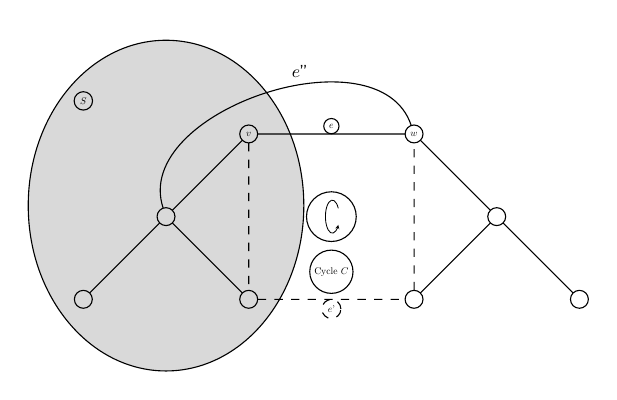
\begin{tikzpicture}[transform shape , scale=0.7]
\draw[fill = gray!30] \boundellipse{-1.5,-1.3}{2.5}{3};
\node [] at(-3,0.6){$S$};
 \node[draw,circle,minimum size= 0.65cm] at (0,0)(A) {$v$};
\node[draw,circle,minimum size= 0.65cm] at (0,-3) (B){};
\node[draw,circle,minimum size= 0.65cm] at (3,-3) (C){};
\node[draw,circle,minimum size= 0.65cm] at (3,0)(D) {$w$};
\node[draw,circle,minimum size= 0.65cm] at (-1.5,-1.5)(E) {};
\node[draw,circle,minimum size= 0.65cm] at (4.5,-1.5) (F){};

\node[draw,circle,minimum size= 0.65cm] at (6,-3)(G) {};
\node[draw,circle,minimum size= 0.65cm] at (-3,-3)(H) {};
\draw [- ,dashed](A) --  (B) --node[below]{$e$'} (C) -- (D);
\draw[-](D)--node[above]{$e$} (A) -- (E) -- (B);
\draw [-] (D) -- (F) -- (C);
\draw (F) -- (G);
\draw[- ] (E) -- (H);
%\draw[-,bend ] (E) -- (D);
  \path[every node/.style={font=\sffamily\small}]
  (E) edge[bend left=90] node [above,pos=0.6] {$e$''} (D);
  \node[rotate=180] at (1.5,-1.5) {\AxisRotator};
    \node[] at (1.5,-2.5) {Cycle $C$};

\end{tikzpicture}

%part 2
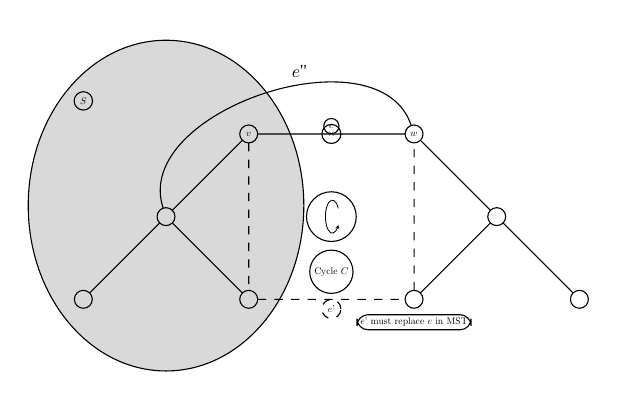
\begin{tikzpicture}[transform shape , scale=0.7]
\draw[fill = gray!30] \boundellipse{-1.5,-1.3}{2.5}{3};
\node [] at(-3,0.6){$S$};
 \node[draw,circle,minimum size= 0.65cm] at (0,0)(A) {$v$};
\node[draw,circle,minimum size= 0.65cm] at (0,-3) (B){};
\node[draw,circle,minimum size= 0.65cm] at (3,-3) (C){};
\node[draw,circle,minimum size= 0.65cm] at (3,0)(D) {$w$};
\node[draw,circle,minimum size= 0.65cm] at (-1.5,-1.5)(E) {};
\node[draw,circle,minimum size= 0.65cm] at (4.5,-1.5) (F){};

\node[draw,circle,minimum size= 0.65cm] at (6,-3)(G) {};
\node[draw,circle,minimum size= 0.65cm] at (-3,-3)(H) {};
\draw [- ,dashed](A) --  (B) --node[below]{$e$'} (C) -- (D);
\draw[-](D)--node[above]{$e$} node[midway]{$\bf{\times}$} (A) -- (E) -- (B);
\draw [-] (D) -- (F) -- (C);
\draw (F) -- (G);
\draw[- ] (E) -- (H);
%\draw[-,bend ] (E) -- (D);
  \path[every node/.style={font=\sffamily\small}]
  (E) edge[bend left=90] node [above,pos=0.6] {$e$''} (D);
  \node[rotate=180] at (1.5,-1.5) {\AxisRotator};
    \node[] at (1.5,-2.5) {Cycle $C$};
\node[draw,rectangle,rounded corners,yshift=-0.5cm] at (C.south)(T) {$e$' must replace $e$ in MST};
\end{tikzpicture}


%%%%%%%%https://gateoverflow.in/39667/gate2016-1-10?show=39680#a39680

\usetikzlibrary{shapes.multipart,chains, positioning}

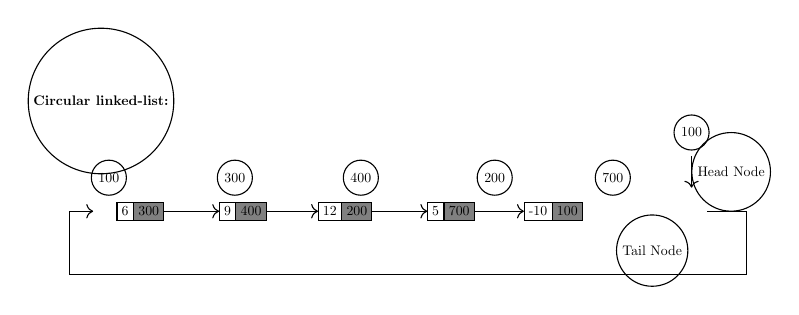
\begin{tikzpicture}
    [
      double link/.style n args=2{% page 726
        on chain,
        rectangle split,
        rectangle split horizontal,
        rectangle split parts=2,
        rectangle split part fill={white,gray},
        draw,
        anchor=center,
        text height=1.5ex,
        node contents={#1\nodepart[fill={gray}]{two}#2},
      },
      start chain=going right,transform shape,scale=1
    ]
   \node []at (-0.5,1.4) {\bf{Circular linked-list:}};
    \node (c) [join={by <-}, double link={6}{300}];
    \node [join={by ->}, double link={9}{400}];
    \node (a) [join={by ->}, double link={12}{200}];
   
    \node [join={by ->}, double link={5}{700}];
    \node (a) [join={by ->}, double link={-10}{100}];
    \draw [->] (7.2,0) -- (7.7,0) -- (7.7,-0.8) -- (-.9,-0.8) -- (-.9,-0.8) -- (-.9,0)-- (-.6,0); 
    \node[above] at (-.4,0.2){100};
 \node[above] at (1.2,0.2){300};
  \node[above] at (2.8,0.2){400};
   \node[above] at (4.5,0.2){200};
    \node[above] at (6,0.2){700};
     \node[] at (6.5,-0.5){Tail Node};
     \node[draw]at (7,1) {100};
    % \draw[->] (7,0.7) --node [right] {head} (7,0.3);
     \draw[->] (7,0.7) --node [right] {Head Node} (7,0.3);
     \end{tikzpicture}

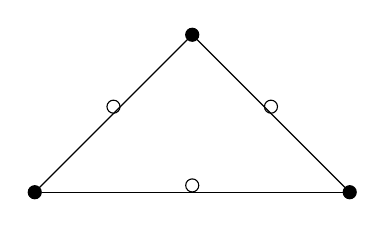
\begin{tikzpicture}
\draw 

(0, 5) node[circle, black,draw, fill = black](a){}
(2, 7) node[circle, black, draw, fill = black](b){}
(4, 5) node[circle, black, draw, fill = black](c){};



\draw[-] (a) -- node[above] {} (b);
\draw[-] (b) -- node[above] {} (c);
\draw[-] (c) -- node[above] {} (a);


\end{tikzpicture}

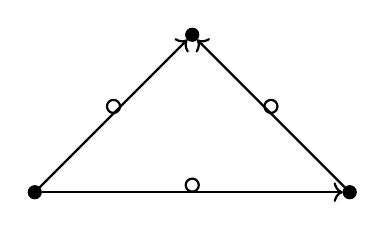
\begin{tikzpicture}
\draw 

(0, 5) node[circle, black,draw, fill = black](a){}
(2, 7) node[circle, black, draw, fill = black](b){}
(4, 5) node[circle, black, draw, fill = black](c){};



\draw[->, thick] (a) -- node[above] {} (b);
\draw[->, thick] (c) -- node[above] {} (b);
\draw[->,thick] (a) -- node[above] {} (c);


\end{tikzpicture}

%https://gateoverflow.in/110918/gate2016-aptitude-set-7-ga-8

  \def\firstcircle{(-210:1.75cm) circle (2.5cm)}
  \def\secondcircle{(-330:1.75cm) circle (2.5cm)}
   \def\thirdcircle{(-210:1.50cm) circle (1.75cm)}
  \def\fourthcircle{(-330:1.50cm) circle (1.75cm)}
 
    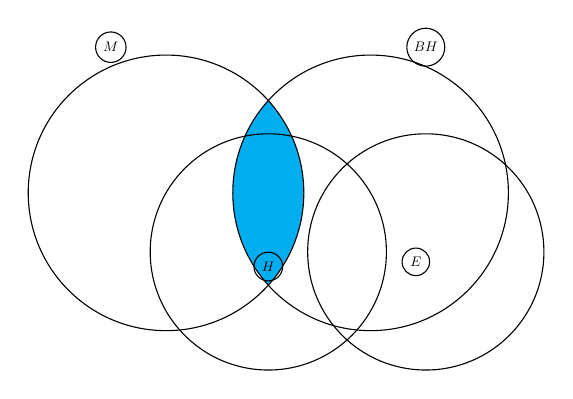
\begin{tikzpicture}
      \begin{scope}
 
    \clip \fourthcircle;
   
    \fill[cyan] \thirdcircle;
    
    
      \end{scope}
     
        
      \draw \firstcircle node[text=black,below] {$H$};
      \draw \secondcircle node [text=black,below left] {$E$};
       \draw \thirdcircle node[text=black ] at (-2,2.6) {$M$};
      \draw \fourthcircle node [text=black] at  (2,2.6){$BH$};
    
    \end{tikzpicture}
  
  
  %
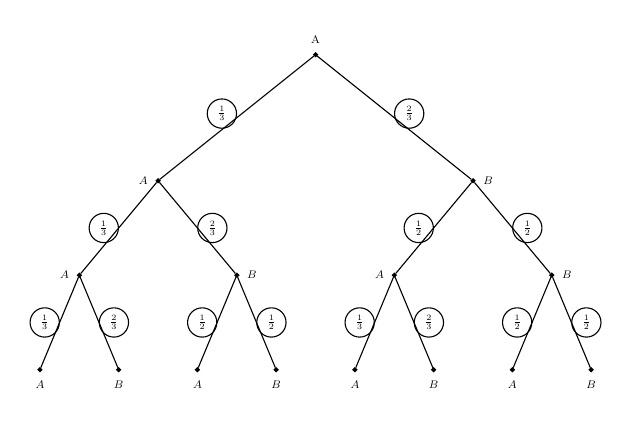
\begin{tikzpicture}
  [
    scale=1,
    font=\footnotesize,
    level 1/.style={level distance=16mm,sibling distance=40mm},
    level 2/.style={level distance=12mm,sibling distance=20mm},
    level 3/.style={level distance=12mm,sibling distance=10mm},
    solid node/.style={circle,draw,inner sep=1,fill=black},
  ]

  \node(0)[solid node, label=A]{}
  child{node(1)[solid node,label=left:{$A$}]{}
    child{node[solid node,label=left:{$A$}]{}
      child{node[solid node,label=below:{$A$}]{} edge from parent node [left]{$\frac{1}{3}$}}
      child{node[solid node,label=below:{$B$}]{} edge from parent node [right]{$\frac{2}{3}$}}
      edge from parent node [left]{$\frac{1}{3}$}
    }
    child{node[solid node,label=right:{$B$}]{}
      child{node[solid node,label=below:{$A$}]{} edge from parent node [left]{$\frac{1}{2}$}}
      child{ node[solid node,label=below:{$B$}]{} edge from parent node [right]{$\frac{1}{2}$}}
      edge from parent node [right]{$\frac{2}{3}$}
    }
    edge from parent node [left, yshift=3]{$\frac{1}{3}$}
  }
  child{node(2)[solid node,label=right:{$B$}]{}
    child{node[solid node,label=left:{$A$}]{}
      child{node[solid node,label=below:{$A$}]{} edge from parent node [left]{$\frac{1}{3}$}}
      child{ node[solid node,label=below:{$B$}]{} edge from parent node [right]{$\frac{2}{3}$}}
      edge from parent node [left]{$\frac{1}{2}$}
    }
    child{node[solid node,label=right:{$B$}]{}
      child{node[solid node,label=below:{$A$}]{} edge from parent node [left]{$\frac{1}{2}$}}
      child{ node[solid node,label=below:{$B$}]{} edge from parent node [right]{$\frac{1}{2}$}}
      edge from parent node [right]{$\frac{1}{2}$}
    }
    edge from parent node [right, yshift=3]{$\frac{2}{3}$}
  };

\end{tikzpicture}


%https://gateoverflow.in/39732/gate-cse-2016-set-1-question-43
\begin{tikzpicture}[>=stealth',shorten >=1pt,node distance=3cm,on grid,auto]
   \node[state,initial,accepting,initial text=] (q_0)     {};
   \node[state] (q_1) [right of = q_0] {};
   \node[state,accepting] (q_2) [right of = q_1] {};
   
   \path[->]
   (q_0) edge [loop above,text width= 2cm]      node {$a,X/XX$ $a,Z/XZ$} ()
         edge                                   node {$b,X/\epsilon$} (q_1)
   (q_1) edge [loop above]       node {$b,X/\epsilon$} ()
         edge                   node {$\epsilon,Z/Z$} (q_2);
\end{tikzpicture}

%https://gateoverflow.in/39562/gate2016-2-16
\begin{tikzpicture}[>=stealth',shorten >=1pt,node distance=2cm,on grid,auto]
   \node[state,initial,initial text=] (q_0)     {};
   \node[state,accepting] (q_1) [right of = q_0] {};
  
   
   \path[->]
   (q_0) edge   node {0,1} (q_1)
   (q_1) edge [loop above] node {0,1} ();
   
\end{tikzpicture}

%https://gateoverflow.in/39598/gate2016-2-46#39695
\begin{tikzpicture}[>=stealth',shorten >=1pt,node distance=2cm,on grid,auto,thick]
    \node       (q)  [left of =A] {\textbf{G1}};
   \node[state] (A)     {D};
   \node[state] (B) [below of=A] {L};
   \node[state] (C) [below right of=B] {E}; 
   \node        (D) [below left of=A] {\textbf{int}};
   \node        (E) [below right of=A] {\textbf{;}};
   \node        (F) [below left of =B] {\textbf{id[}};
   \node        (G) [below left of =C] {\textbf{num][}};
   \node[state] (H) [below  of =C] {E};
   \node        (I) [below of=H] {\textbf{num]}};
  
 \path[->]
 (A) edge                node {} (E)
     edge                node {} (D)
     edge                node {} (B)
 (B) edge                node {} (F)
     edge                node {} (C)
 (C) edge                node {} (G)
     edge                node {} (H)
 (H) edge                node {} (I);
   
\end{tikzpicture}

%https://gateoverflow.in/39598/gate2016-2-46#39695
\begin{tikzpicture}[>=stealth',shorten >=1pt,node distance=2cm,on grid,auto,thick]
    \node       (q)  [left of =A] {\textbf{G2}};
   \node[state] (A)     {D};
   \node[state] (B) [below of=A] {L};
   \node[state] (C) [below right of=B] {E}; 
   \node        (D) [below left of=A] {\textbf{int}};
   \node        (E) [below right of=A] {\textbf{;}};
   \node        (F) [below left of =B] {\textbf{id}};
   \node [state]       (G) [below left of =C] {E};
   \node         (H) [below  of =C] {\textbf{[num]}};
   \node        (I) [below of=G] {\textbf{[num]}};
  
 \path[->]
 (A) edge                node {} (E)
     edge                node {} (D)
     edge                node {} (B)
 (B) edge                node {} (F)
     edge                node {} (C)
 (C) edge                node {} (G)
     edge                node {} (H)
 (G) edge                node {} (I);
   
\end{tikzpicture}


%https://gateoverflow.in/39535/gate-cse-2016-set-2-question-ga-10

\begin{tikzpicture}

\newcommand*{\XAxisMin}{-4}
\newcommand*{\XAxisMax}{4}
\newcommand*{\YAxisMin}{-2.5}
\newcommand*{\YAxisMax}{2.5}
 %axis on top=true,
\begin{axis}[
%axis equal=true,
ymajorgrids,
 width=0.6\linewidth,
  height=0.4\linewidth,
   line width=1.5,
    axis y line=center, axis x line=middle,
    xmin=\XAxisMin, xmax=\XAxisMax, ymin=\YAxisMin, ymax=\YAxisMax, 
    xtick=data,
ytick={-2.5,-2,-1.5,-1,-0.5,0,0.5,1,1.5,2,2.5},
xtick={-4,-3,-2,-1,0,1,2,3,4},
inner axis line style={-},
    xlabel={$x$},
     ylabel={$f(x)$},
] 

 \addplot[blue] coordinates
      {(-3,-2) (1,2) (3,0)};
     

\end{axis} 
\end{tikzpicture} 

%%https://gateoverflow.in/108289/gate2016-me-2-ga-5?show=216978#a216978
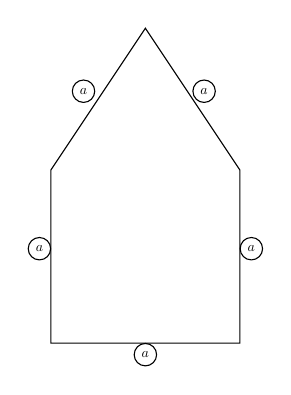
\begin{tikzpicture}[scale = 0.8]
\draw[] (0,2.75)-- (0,0) -- (3,0) -- (3,2.75) -- (1.5,5) -- (0,2.75);

\node[below] at (1.5,0){$a$};
\node[right] at (3,1.5){$a$};
\node[left] at (0,1.5){$a$};
\node[left] at (0.70,4){$a$};
\node[right] at (2.25,4){$a$};
\end{tikzpicture}






%https://gateoverflow.in/302808/gate-cse-2019-question-40#327311
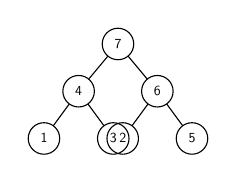
\begin{tikzpicture}[level/.style={sibling distance=25mm/#1},level 2/.style={sibling distance=22mm},font = \sffamily,scale=0.4]
    \node [draw, circle,minimum size= 8mm]{7}
        child {node [draw, circle,minimum size= 8mm]{4}
            child {node [draw, circle,minimum size= 8mm]{1}}
            child {node [draw, circle,minimum size= 8mm]{3}}
        }
        child {node [draw, circle,minimum size= 8mm]{6}
            child {node [draw, circle,minimum size= 8mm]{2}}
            child {node [draw, circle,minimum size= 8mm]{5}}
        }
    ;
\end{tikzpicture}

%https://gateoverflow.in/302808/gate-cse-2019-question-40#327311
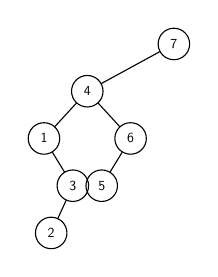
\begin{tikzpicture}[level/.style={sibling distance=55mm/#1},font = \sffamily,scale=0.4]    
    \node [draw, circle,minimum size= 8mm]{7}
        child {node [draw, circle,minimum size= 8mm]{4}
            child {node [draw, circle,minimum size= 8mm]{1}
                child[missing]{}
                child{node [draw, circle,minimum size=8mm]{3}
                    child{node [draw, circle,minimum size=8mm]{2}}
                    child[missing]{}
                }
            }
            child {node [draw, circle,minimum size= 8mm]{6}
                child{node [draw, circle,minimum size=8mm]{5}}
                child[missing]{}
            }
        }
        child[missing] {}
    ;
\end{tikzpicture}

%https://gateoverflow.in/302802/gate-cse-2019-question-46?show=323153
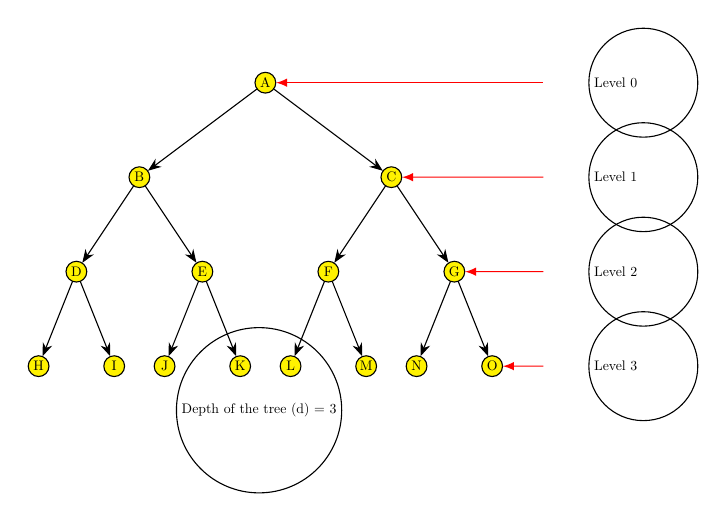
\begin{tikzpicture}[->,>=stealth,scale=0.8, level/.style={circle,draw,>=Stealth},
level 1/.style={sibling distance=40mm},level 2/.style={sibling distance=20mm},level 3/.style={sibling distance=12mm},minimum size=0.50cm,iv/.style={draw,rectangle,minimum size=15pt,inner sep=0pt,text=black},ev/.style={draw,circle,minimum size=15pt,inner sep=0pt,text=black,fill=yellow}]
\node[ev,name=A]{A}  
               child {node[ev]{B}
               child {node[ev]{D}
               child {node[ev]{H}}
               child {node[ev]{I}}
               }
               child {node[ev]{E}
               child {node[ev]{J}}
               child {node[ev]{K}}
               }
               }
               child {node[ev,name=C]{C}
               child {node[ev]{F}
               child {node[ev]{L}}
               child {node[ev]{M}}
               }
               child {node[ev,name=G]{G}
               child {node[ev]{N}}
               child {node[ev,name=O]{O}}
               }
};
%let \p1 = (A);
\draw[<-,>=latex,shorten >=2pt,node distance=2cm,on grid,auto,color=red] (A) -- (A -| 4.5,0);
\draw[<-,>=latex,shorten >=2pt,node distance=2cm,on grid,auto,color=red](C) -- (C -| 4.5,0);
\draw[<-,>=latex,shorten >=2pt,node distance=2cm,on grid,auto,color=red](G) -- (G-|4.5,0);
\draw[<-,>=latex,shorten >=2pt,node distance=2cm,on grid,auto,color=red](O) -- (O-|4.5,0);
\node [text width=2.5cm,align=left] at (A-|6,0.0) {Level $0$};
\node [text width=2.5cm,align=left] at (C-|6,0) {Level $1$};
\node [text width=2.5cm,align=left] at (G-|6,0) {Level $2$};
\node [text width=2.5cm,align=left] at (O-|6,0) {Level $3$};
\node at (-0.1,-5.2) {Depth of the tree (d) = $3$};
\end{tikzpicture}

%https://gateoverflow.in/302800/gate2019-48?show=303078#a303078

    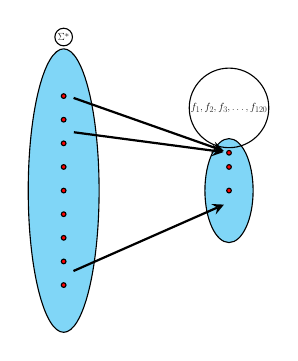
\begin{tikzpicture}[
    >=stealth,scale=0.3,transform shape,
    bullet/.style={
        fill=black,
        circle,
        minimum width=1pt,
        inner sep=1pt
    },
    projection/.style={
        ->,
        thick,
        shorten <=2pt,
        shorten >=2pt
    },
    every fit/.style={
        ellipse,
        draw,
        inner sep=0pt
    },
        setA/.style={fill=red,circle,inner sep=4pt}
    ]
 
  

    \draw[fill=cyan!50] (0,2.5) ellipse (1.5cm and 6cm);
    \draw[fill=cyan!50] (7,2.5) ellipse (1.02cm and 2.2cm);
   \node[font=\Huge] at (0,9){$\Sigma^*$};
\node[font=\Huge] at (7,6) {${f_1,f_2,f_3,\ldots,f_{120}}$};
  \node[setA] (a) at (0,6.5) {};
    \node[setA,below of = a] (b) at (0,6) {};
      \node[setA,below of = b] (c) at (0,5) {};
        \node[setA,below of = c] (d) at (0,4) {};
          \node[setA,below of = d] (e) at (0,3) {};
            \node[setA,below of = e] (f) at (0,2) {}; 
            \node[setA,below of = f] (g) at (0,1) {};
              \node[setA,below of = g] (h) at (0,0) {}; 
            \node[setA,below of = h] (i) at (0,-1) {};

 \node[setA] (a) at (7,4.1) {};
    \node[setA,below of = a] (b) at (7,4) {};
      \node[setA,below of = b] (c) at (7,3) {};
 
    \draw[projection] (0.2,6.5) -- (7,4.1);
     \draw[projection] (0.2,5) -- (7,4.1);
      \draw[projection] (0.2,-1) -- (7,2);
 

   % \draw[projection] (0.3,2.5) -- (3.7,2.5);
   % \draw[projection] (4.3,2.5) -- (7.7,2.5);
    \end{tikzpicture}
 


  
 %%%%% ugcnet2-june2019 By Lakshman Patel %% 
%https://gateoverflow.in/316278/ugcnet-june-2019-ii-1?show=316349#a316349
\tikzset{state/.style={draw,circle}}
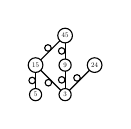
\begin{tikzpicture}[shorten >=0.01pt,node distance = 1.5cm,auto,scale = 0.5,transform shape]

\node[](1){5};
\node[](2)[right of = 1]{3};
\node[](3)[above of = 1]{15};
\node[](4)[above of = 2]{9};
\node[](5)[above of = 4]{45};
\node[](6)[right of = 4]{24};

\path (1) edge[] node {}(3);
\path (2) edge[] node {}(3);
\path (2) edge[] node {}(4);
\path (2) edge[] node {}(6);
\path (3) edge[] node {}(5);
\path (4) edge[] node {}(5);
\end{tikzpicture}


%https://gateoverflow.in/316188/ugcnet-june-2019-ii-91
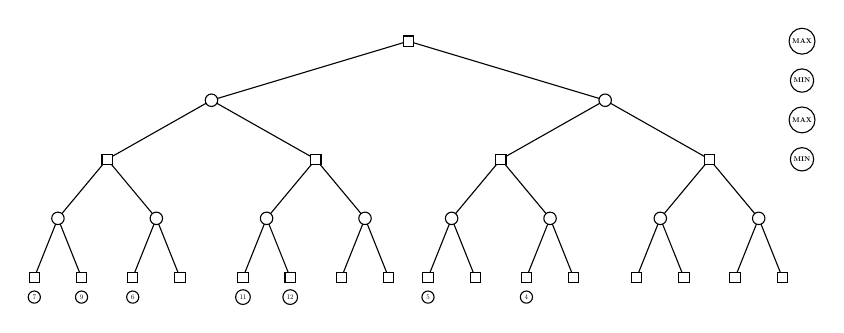
\begin{tikzpicture}[cv/.style={minimum size = 18pt,inner sep=2pt,draw,circle},iv/.style={minimum size = 15pt,inner sep=1.5pt,draw,rectangle},level 1/.style={sibling distance=10cm},level 2/.style={sibling distance=5.3cm},level 3/.style={sibling distance=2.5cm},level 4/.style={sibling distance=1.2cm},transform shape,scale = 0.5]
\node[iv]{}
    child {node[cv]{}
          child {node[iv]{}
                 child {node[cv]{}
                       child {node[iv]{}}
                       child {node [iv]{}}}
                 child {node [cv]{}
                       child {node[iv]{}}
                       child {node [iv]{}}}}
          child {node [iv]{}
                child {node[cv]{}
                       child {node[iv]{}}
                       child {node [iv]{}}}
                 child {node [cv]{}
                       child {node[iv]{}}
                       child {node [iv]{}}}}}
    child {node [cv]{}
          child {node[iv]{}
                 child {node[cv]{}
                       child {node[iv]{}}
                       child {node [iv]{}}}
                 child {node [cv]{}
                       child {node[iv]{}}
                       child {node [iv]{}}}}
          child {node [iv]{}
                child {node[cv]{}
                       child {node[iv]{}}
                       child {node [iv]{}}}
                 child {node [cv]{}
                       child {node[iv]{}}
                       child {node [iv]{}}}}};
\node at (10,0) {$\textbf{MAX}$};
\node at (10,-1) {$\textbf{MIN}$};   
\node at (10,-2) {$\textbf{MAX}$};   
\node at (10,-3) {$\textbf{MIN}$};

\node at (-9.5,-6.5) {7}; 
\node at (-8.3,-6.5) {9};
\node at (-7,-6.5) {6};
\node at (-4.2,-6.5) {11};
\node at (-3,-6.5) {12};
\node at (0.5,-6.5) {5};
\node at (3,-6.5) {4}; 

\end{tikzpicture}

%https://gateoverflow.in/316204/ugcnet-june-2019-ii-75?show=317159#a317159
\begin{tikzpicture}[shorten >=0.01pt,->,>=latex,node distance = 2cm,auto,scale = 0.5,transform shape]

\node[state,initial,initial text = ](1){P};
\node[state](2)[right of = 1]{Q};
\node[state,accepting](3)[right of = 2]{R};

\path (1) edge[loop above] node {a}(1);
\path (1) edge[] node {b}(2);
\path (2) edge[] node {a,b}(3);

\end{tikzpicture}

%https://gateoverflow.in/316245/ugcnet-june-2019-ii-34?show=317133#a317133
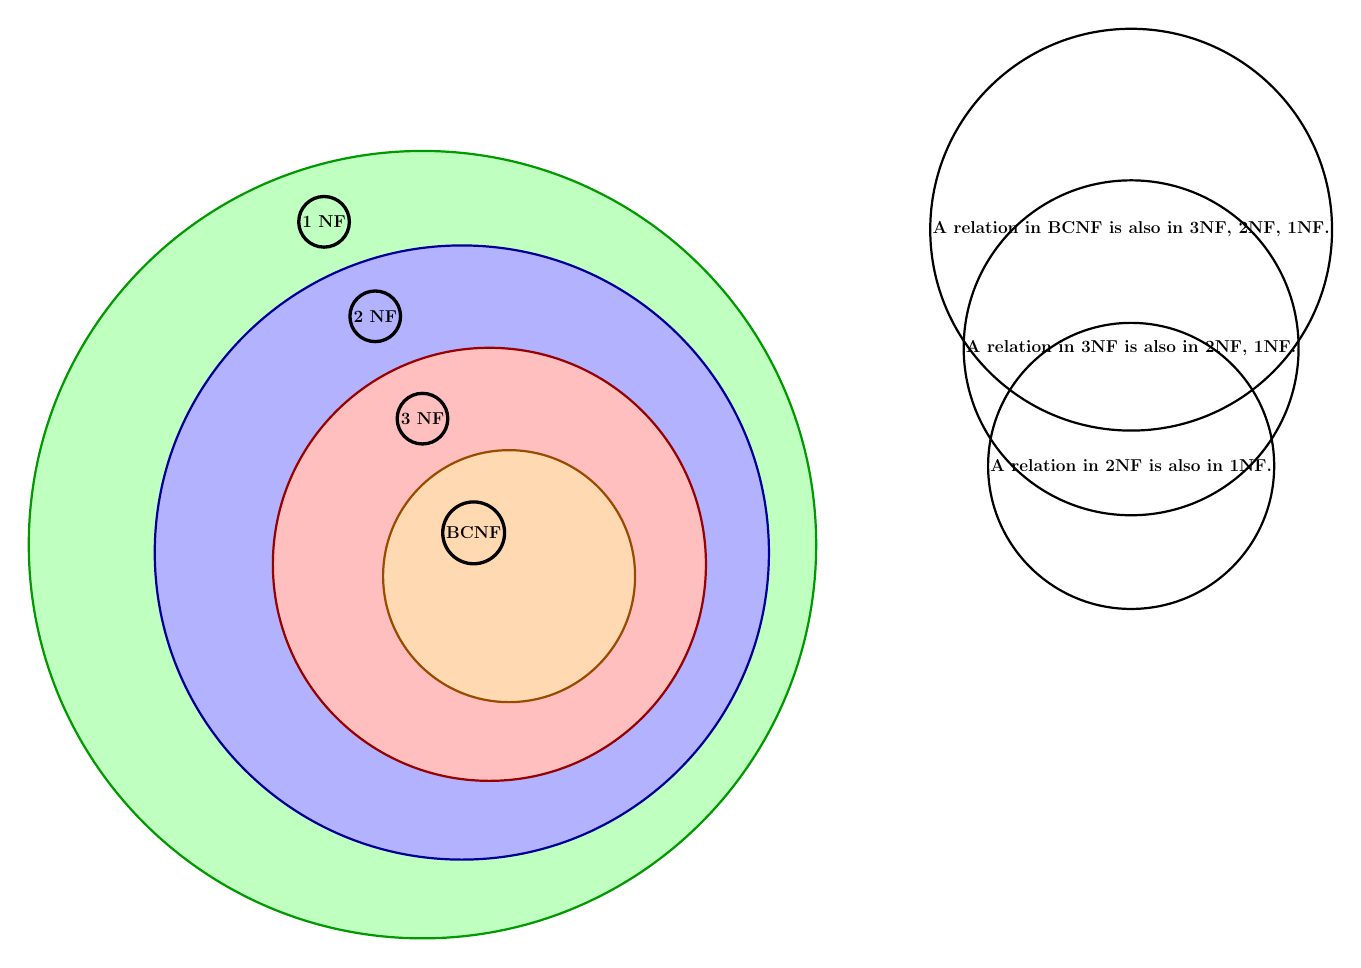
\begin{tikzpicture}[scale = 0.5,thick,transform shape]
\draw[color=green!60!black,fill=green!25!white] (0,0) circle (10cm);
\draw[color=blue!60!black,fill = blue!30!white] (1,-0.2) circle (7.8cm);
\draw[color=red!60!black,fill = red!25!white] (1.7,-0.5) circle (5.5cm);
\draw[color=orange!60!black,fill = orange!30!white] (2.2,-0.8) circle (3.2cm);

\node[very thick] at (1.3,0.3){\Huge{\textbf{BCNF}}};
\node[very thick] at (0,3.2) {\Huge{\textbf{3 NF}}};
\node[very thick] at (-1.2,5.8) {\Huge{\textbf{2 NF}}};
\node[very thick] at (-2.5,8.2) {\Huge{\textbf{1 NF}}};

\node at (18,8) {\Huge{\textbf{A relation in BCNF is also in 3NF, 2NF, 1NF.}}};
\node at (18,5) {\Huge{\textbf{A relation in 3NF is also in 2NF, 1NF.}}};
\node at (18,2) {\Huge{\textbf{A relation in 2NF is also in 1NF.}}};
\end{tikzpicture}

%https://gateoverflow.in/313448/gate2019-ce-1-ga-10?show=314121#a314121 
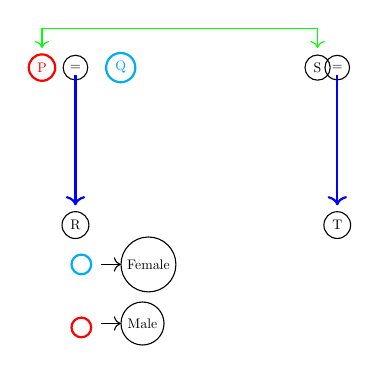
\begin{tikzpicture}[scale=0.5]
\node[thick,draw,circle,color= cyan,minimum size= 0.5cm] at (-2,0) {Q} ;
\node[thick,draw,color= red,minimum size= 0.5cm] at (-4,0) {P} ;
\node[] at (-3.15,0) {=};
\node[] at (3,0) {S};
\node[] at (3.5,0) {=};
\node[] at (3.5,-4) {T};
\node[] at (-3.15,-4) {R};
\draw[<->,color=green] (-4,0.5) -- (-4,1) -- (3,1) -- (3,0.5);
\draw[->,thick,color=blue] (-3.15,-0.2) -- (-3.15,-3.5) ;
\draw[->,thick,color= blue] (3.5,-0.2) -- (3.5,-3.5) ;
\node[thick,draw,circle,color= cyan,minimum size= 0.5cm] at (-3,-5) {} ;
\node[thick,draw,color= red,minimum size= 0.5cm] at (-3,-6.6) {} ;
\draw[->] (-2.5,-5)--(-2,-5) node[right]{Female};
\draw[->] (-2.5,-6.5)--(-2,-6.5) node[right]{Male};
\end{tikzpicture}


%https://gateoverflow.in/302866/gate2019-ga-7
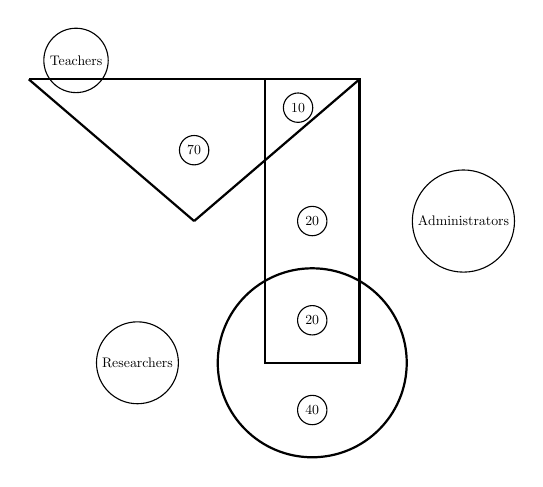
\begin{tikzpicture}[scale=0.6]
\draw[black,thick] (0,0) -- (-7,0);
\draw[black,thick] (0,0) -- (-3.5,-3);
\draw[black,thick] (-7,0) -- (-3.5,-3);
\draw [black,thick] (0,0) rectangle (-2,-6);
\draw [black, thick] (-1,-6) circle [radius=2];
\node at (-6,0.4) {Teachers};
\node at (2.2,-3) {Administrators};
\node at (-4.7,-6) {Researchers};
      
\node at (-3.5,-1.5) {$70$};
\node at (-1.3,-0.6) {$10$};
\node at (-1,-3) {$20$};
\node at (-1,-5.1) {$20$};
\node at (-1,-7) {$40$};

\end{tikzpicture}

 %
   % this is to allow the fork right path

%https://gateoverflow.in/302807/gate2019-41?show=303043#a303043

\usetikzlibrary{positioning}
\tikzset{
  gray box/.style={
    fill=white!20,
    draw=black,
    minimum width={2*#1ex},
    minimum height={3em},
  },
  annotation/.style={
    anchor=north,
  }
}
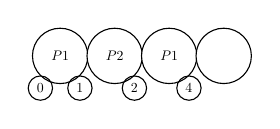
\begin{tikzpicture}[node distance=-0.5pt]
  \node [gray box=1] (p1) {\(P1\)}; ;

  \node [gray box=1, right=of p1] (p2) {\(P2\)};
  \node [gray box=3.5, right=of p2] (p3) {\(P1\)};
    \node [gray box=4.5, right=of p3] (p4) {};
 
 \node [annotation] at (p1.south west) {0};
  \node [annotation] at (p1.south east) {1};
 \node [annotation] at (p2.south east) {2};
  \node [annotation] at (p3.south east) {4};
%  \node [annotation] at (p4.south east) {};


\end{tikzpicture}
%https://gateoverflow.in/302798/gate2019-50?show=302798#q30279
 
  \begin{karnaugh-map}[4][4][1][][][baseline=(current bounding box.north),scale=.3]
        \minterms{0,2,8,10,7,5,13,15}
      
        \autoterms[0]
        \implicantedge{1}{3}{9}{11}
        \implicantedge{4}{12}{6}{14}
       % \implicant{4}{5}
        \node at (-0.25,4.7) {CD};           % row name
        \node at (-0.6,4.15) {AB};            % column name
        \draw[ultra thin] (0,4) -- (-1,4.75);  % diagonal line
    \end{karnaugh-map}
    
    
   

%https://gateoverflow.in/302801/gate2019-47?show=303770#a303770
\begin{figure}

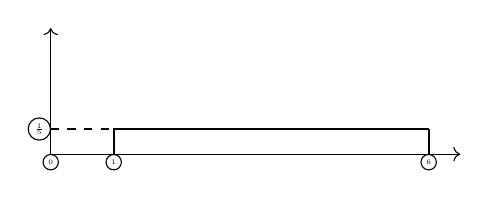
\begin{tikzpicture}[scale=0.8]
\tiny
\tiny
\draw [->](0,0) -> (6.5,0);

\draw [->](0,0) -- (0,2);
\draw [thick] (1,0)--(1,0.4) -- (6,0.4);
\draw [dashed] (0,0.4)--(1,0.4);
\draw [thick] (6,0.4)--(6,0);

\node [below] at (0,0) {$0$};

\node [below] at (1,0) {$1$};

\node [below] at (6,0) {$6$};

\node [left] at (0,0.4) {$1 \over 5 $};
\end{tikzpicture}

\end{figure}


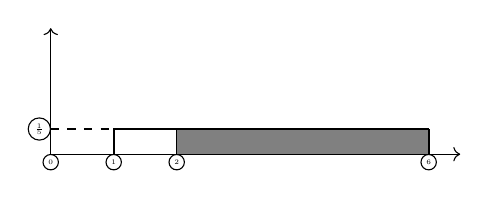
\begin{tikzpicture}[scale=0.8]

\tiny

\tiny

\draw[->] (0,0) -- (6.5,0);

\draw[->] (0,0) -- (0,2);
\draw[thick] (2,0.4) -- (2,0);

\draw [thick] (1,0)--(1,0.4) -- (6,0.4);

\draw [dashed] (0,0.4)--(1,0.4);

\draw [thick] (6,0.4)--(6,0);


\node [below] at (0,0) {$0$};
\node [below] at (2,0) {$2$};
\node [below] at (1,0) {$1$};

\node [below] at (6,0) {$6$};

\draw[fill=gray]  (2,0) -- (2,0.4) -- (6,0.4) -- (6,0) -- cycle;

\node [left] at (0,0.4) {$1 \over 5 $};

\end{tikzpicture}




%%%%%%%%%%https://gateoverflow.in/313438/gate2019-ce-1-ga-3?show=314085#a314085

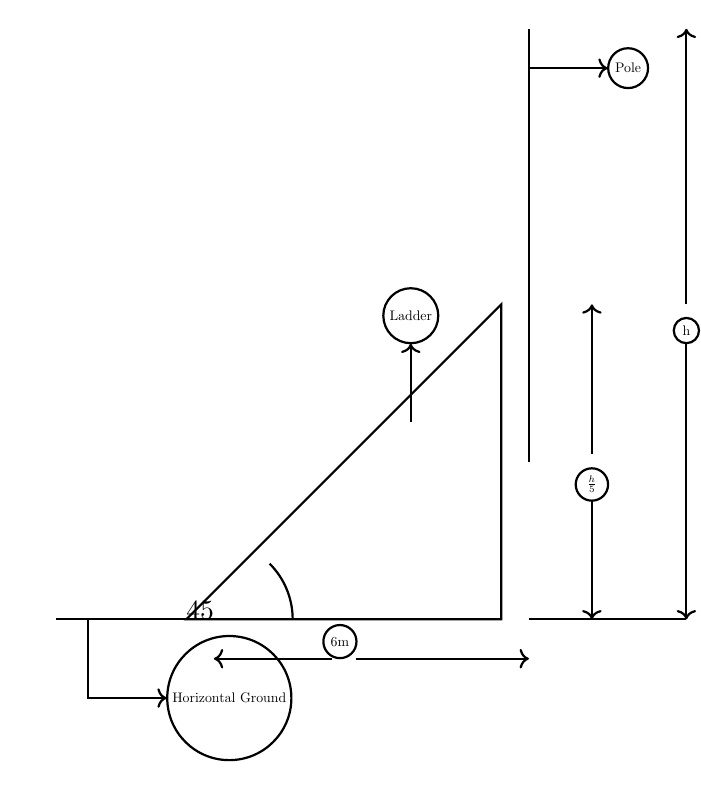
\begin{tikzpicture}[thick]

\coordinate (O) at (4,0);
\coordinate (A) at (0,0);
\coordinate (B) at (4,4);
\draw (O)--(A)--(B)--cycle;

\tkzLabelAngle[pos = 0.35](A,O,B){}


\tkzLabelAngle[pos = 0.6](B,A,O){$45$}

\tkzLabelAngle[pos = 0.5](O,B,A){}
\draw[-] (4,2) -- (4,7.5);
\draw[-] (0,0) -- (-2,0);
\draw[-] (4,0) -- (6,0);
\draw[->] (4,7) -- (5,7);
\node[right] at (5,7){Pole};
\draw[->] (2.5,2.5) -- (2.5,3.5);
\node[above] at (2.5,3.5){Ladder};

\draw[<-](6,0) -- (6,3.5);
\node[above] at (6,3.5){h};
\draw[->](6,4)-- (6,7.5);


\draw[<-](0,-0.5) -- (1.5,-0.5);
\node[above] at (1.6,-.5){6m};
\draw[->](1.8,-0.5)-- (4,-0.5);


\draw[<-](4.8,0) -- (4.8,1.5);
\node[above] at (4.8,1.5){$\frac{h}{5}$};
\draw[->](4.8,2.1)-- (4.8,4);




\draw[->] (-1.6,0) |- (-.6,-1);
\node[right] at (-.6,-1){Horizontal Ground };

  \draw (1,0) arc (0:45:1);
%   \begin{axis}
 
%   \addplot [thick,color=blue,,mark=o,fill=blue, 
%                     fill opacity=0.05] coordinates {
%           (-2,0)
%             (-2, -.5)
%             (6, -.5)
%             (6,0) };
% \end{axis}

\end{tikzpicture}

%https://gateoverflow.in/302818/gate2019-30?show=302818#q302818

\begin{tikzpicture}[label distance=1mm]
\node (A) at (0, 0)  {\small{$f_1$}};
\node (B) at (0, -0.36) {\small{$f_2$}};
\node (C) at (0, -1.8) {\small{$f_3$}};
\node (D) at (5.5, -1.6) {\small{$f$}};
\node[and gate US, draw, anchor=input 1] at ($(A) + (1.0, 0.0)$) (and1) {AND};
\node[xor gate US, draw, anchor=input 1] at ($(C) + (3.2, 0.4)$) (xor1) {XOR};
\draw (A) -- (and1.input 1);
\draw (B) -- (and1.input 2);
\draw (and1.output) -- ([xshift=0.5cm]and1.output) |- (xor1.input 1);
\draw (C) -- (xor1.input 2);
\draw (xor1.output) -- ([xshift=0.8cm]xor1.output);
\end{tikzpicture}


%%https://gateoverflow.in/313528/gate2019-ec-ga-7
%first image
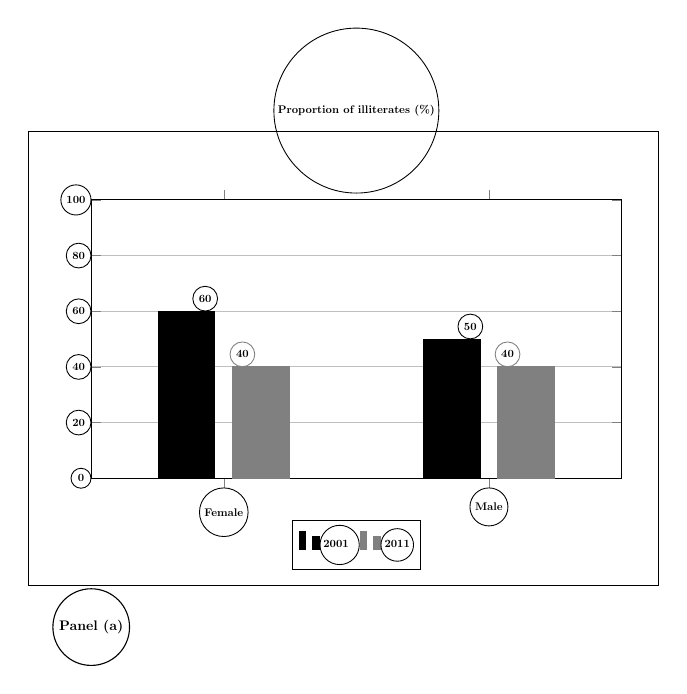
\begin{tikzpicture}[scale = 0.8,font = \bfseries]
\begin{axis}[
ybar=8pt, %space between adjacent bars is 0
enlarge x limits=0.5,
enlarge y limits=false,
legend style={at={(0.5,-0.15),ybar=area},
anchor=north,legend columns=-1.15},
title = {Proportion of illiterates (\%)},
ymajorgrids = true,
%xmajorgrids = true,
ylabel=,
symbolic x coords={Female, Male},
xtick=data,
ytick={0,20,...,80,100},
nodes near coords,
bar width=0.90cm,
every node near coord/.append style={font=\boldmath},
nodes near coords align={vertical},
every x tick label/.append style={font=\bfseries},
every y tick label/.append style={font=\boldmath},
%tick label style={font=\boldmath}, 
label style={color=black,font=\bfseries},
width=10cm,
height=6cm,
ymax=100,
ymin=0
]
\addplot
[fill=black,draw=black]
coordinates {(Female,60) (Male,50)};
\addplot
[fill=gray,draw=gray]
coordinates {(Female,40) (Male,40)};
\legend{2001\;\;,2011}
\end{axis}

\draw[] (-1,-1.70) rectangle (9,5.5);
\node[below] at (0,-1.75) {Panel (a)};

\end{tikzpicture}

%second image

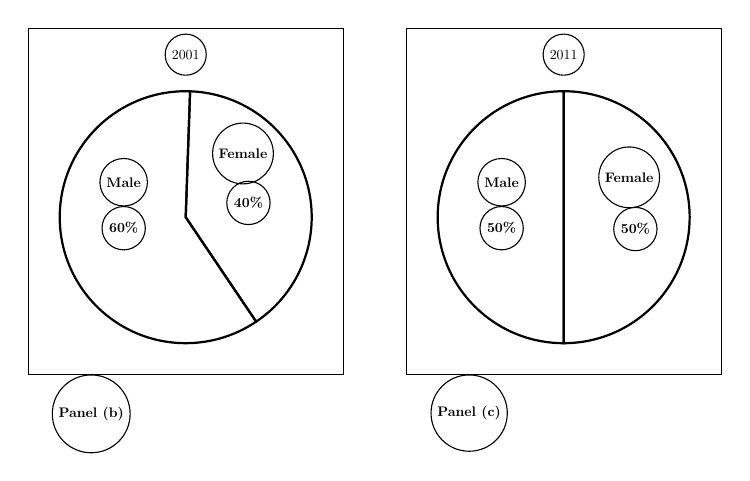
\begin{tikzpicture}[scale = 0.8]

\begin{scope}
\draw[draw=black,line width=0.15mm,thick] (0,0) -- (-56:2cm) arc[start angle=-56,end angle=88,radius=2cm] -- cycle;

\draw[draw=black,line width=0.15mm,thick] (0,0) -- (88:2cm) arc[start angle=88,end angle=304,radius=2cm] -- cycle;

\node[below] at (30:1.15cm) {\textbf{40\%}};
\node[above] at (30:1.05cm) {\textbf{Female}};

\node[below] at (170:1cm) {\textbf{60\%}};
\node[above] at (170:1cm) {\textbf{Male}};

\draw[] (-2.5,-2.5) rectangle (2.5,3);
\node[above] at (0,2.25) {$2001$};
\node[below] at (-1.5,-2.5) {\textbf{Panel (b)}};

\end{scope}

\begin{scope}[xshift = 6cm]
\draw[draw=black,line width=0.15mm,thick] (0,0) -- (-90:2cm) arc[start angle=-90,end angle=90,radius=2cm] -- cycle;

\draw[draw=black,line width=0.15mm,thick] (0,0) -- (90:2cm) arc[start angle=90,end angle=270,radius=2cm] -- cycle;

\node[below] at (8:1.15cm) {\textbf{50\%}};
\node[above] at (8:1.05cm) {\textbf{Female}};

\node[below] at (170:1cm) {\textbf{50\%}};
\node[above] at (170:1cm) {\textbf{Male}};

\draw[] (-2.5,-2.5) rectangle (2.5,3);
\node[above] at (0,2.25) {$2011$};
\node[below] at (-1.5,-2.5) {\textbf{Panel (c)}};
\end{scope}

\end{tikzpicture}




% https://gateoverflow.in/302846/gate-cse-2019-question-2

\begin{tikzpicture}[minimum height=2cm,scale=2] 
        \node[and gate US, draw,logic gate inputs=nniin] (A) {}; 
        \foreach \a [evaluate=\a as \aeval using int(6-\a)]in {1,...,5}
        {
            \draw (A.input \a -| -1,0)node [left]{$A_{1\aeval}$} -- (A.input \a) ; 
            }
        \draw (A.output) -- ([xshift=0.8cm]A.output) node [anchor=west]{CS};
    \end{tikzpicture} 

%%%%https://gateoverflow.in/302799/gate-cse-2019-question-49?show=303878#a303878
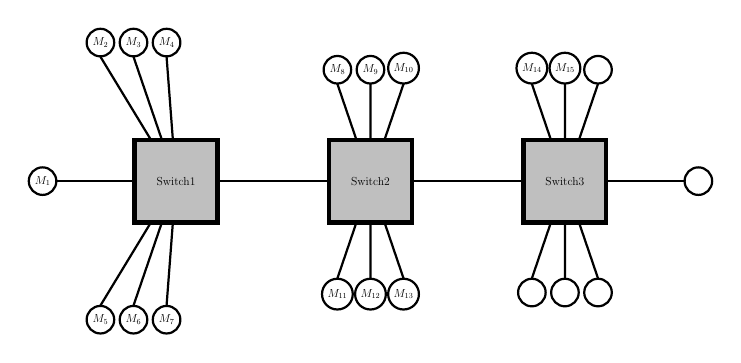
\begin{tikzpicture}[scale=0.7,transform shape,font=\large]

%%%Switch1
\node[rectangle,draw,minimum width = 30mm,minimum height = 30mm,anchor=center,fill=lightgray,ultra thick] (n1) {Switch1};
\node[circle,draw,minimum size = 1cm,thick,left=1.4cm of n1] (c1) {$M_1$};
\node[circle,draw,minimum size = 1cm,thick, above= 2cm of c1, xshift=2.1cm] (c2) {$M_2$};
\node[circle,draw,minimum width = 1cm,thick, above= 2cm of c1, xshift=3.3cm] (c3) {$M_3$};
\node[circle,draw,minimum width = 1cm,thick, above= 2cm of c1, xshift=4.5cm] (c4) {$M_4$};

\node[circle,draw,minimum width = 1cm,thick, below= 2cm of c1, xshift=2.1cm] (c5) {$M_5$};
\node[circle,draw,minimum width = 1cm, thick, below= 2cm of c1, xshift=3.3cm] (c6) {$M_6$};
\node[circle,draw,minimum width = 1cm,thick, below= 2cm of c1, xshift=4.5cm] (c7) {$M_7$};

\draw [ thick] (n1) -- (c1);
\draw [ thick] (n1) -- (c2.south);
\draw [ thick] (n1) -- (c3.south);
\draw [thick] (n1) -- (c4.south);
\draw [ thick] (n1) -- (c5.north);
\draw [thick] (n1) -- (c6.north);
\draw [ thick] (n1) -- (c7.north);
%%%Switch2
\node[rectangle,draw,minimum width = 30mm,minimum height = 30mm,anchor=center,right=20mm of n1,fill=lightgray,ultra thick] (n2) {Switch2};

\node[circle,draw, ,minimum size = 1cm,thick,above= 1cm of n2,xshift=-1.2cm] (c8) {$M_8$};
\node[circle,draw,minimum width = 1cm, thick, above= 1cm of n2, xshift=0cm] (c9) {$M_9$};
\node[circle,draw,minimum size = 1cm,thick, above= 1cm of n2, xshift=1.2cm] (c10) {$M_{10}$};

\node[circle,draw,minimum width = 1cm,thick, below= 1cm of n2, xshift=-1.2cm] (c11) {$M_{11}$};
\node[circle,draw,minimum width = 1cm,thick, below= 1cm of n2, xshift=0cm] (c12) {$M_{12}$};
\node[circle,draw,minimum width = 1cm,thick, below= 1cm of n2, xshift=1.2cm] (c13) {$M_{13}$};

\draw [thick] (n2) -- (c8.south);
\draw [ thick] (n2) -- (c9.south);
\draw [ thick] (n2) -- (c10.south);
\draw [thick] (n2) -- (c11.north);
\draw [thick] (n2) -- (c12.north);
\draw [thick] (n2) -- (c13.north);

%%%Switch3
\node[rectangle,draw,minimum width = 30mm,minimum height = 30mm,anchor=center,right=20mm of n2,fill=lightgray,ultra thick] (n3) {Switch3};

\node[circle,draw, ,minimum size = 1cm,thick,above= 1cm of n3,xshift=-1.2cm] (c14) {$M_{14}$};
\node[circle,draw,minimum width = 1cm,thick, above= 1cm of n3, xshift=0cm] (c15) {$M_{15}$};
\node[circle,draw,minimum size = 1cm,thick, above= 1cm of n3, xshift=1.2cm] (c16) {};

\node[circle,draw,minimum width = 1cm,thick, below= 1cm of n3, xshift=-1.2cm] (c17) {};
\node[circle,draw,minimum width = 1cm,thick, below= 1cm of n3, xshift=0cm] (c18) {};
\node[circle,draw,minimum width = 1cm,thick, below= 1cm of n3, xshift=1.2cm] (c19) {};

\node[circle,draw,minimum size = 1cm,thick,right=1.4cm of n3] (c20) {};

\draw [thick] (n3) -- (c14.south);
\draw [thick] (n3) -- (c15.south);
\draw [ thick] (n3) -- (c16.south);
\draw [thick] (n3) -- (c17.north);
\draw [thick] (n3) -- (c18.north);
\draw [ thick] (n3) -- (c19.north);
\draw [thick] (n3.east) -- (c20.west);

\draw [thick] (n1.east) -- (n2.west);
\draw [thick] (n2.east) -- (n3.west);

\end{tikzpicture}

%https://gateoverflow.in/118703/gate-cse-2017-set-1-question-04
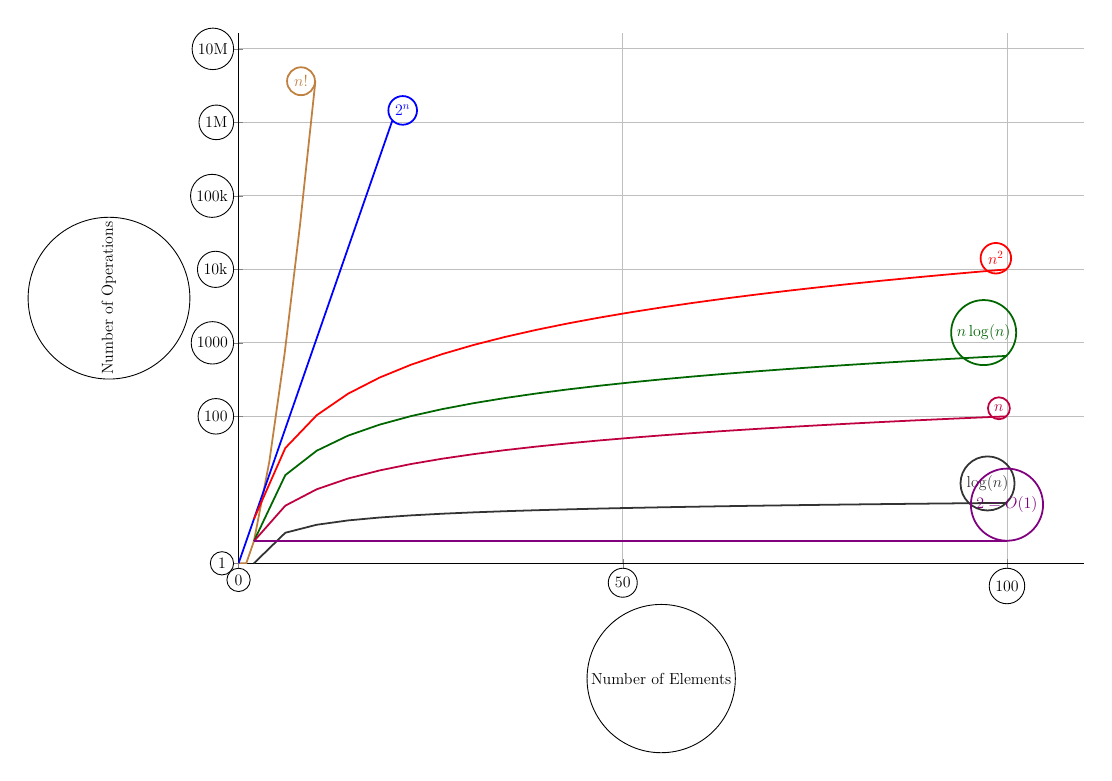
\begin{tikzpicture}[scale=0.8]
\begin{semilogyaxis}[height=10cm,width=15cm,
        scaled ticks=false,font=\Large,
        log ticks with fixed point,
        ylabel near ticks,
ytick={1,100,1000,10000,100000,1000000,10000000,100000000,1000000000},
         max space between ticks=1000pt,
        %try min ticks=5,
       grid=both,
        axis lines=left,
        axis line style=-,
        enlargelimits={upper=0.3},
        ylabel = Number of Operations,
        xlabel = Number of Elements,
        ymin=1,ymax=,xmin=0,xmax=100,domain=2:100,
        log basis y =2,
        yticklabels={1,100,1000,10k,100k,1M,10M,100M,1G,10G,100G},
       % ylabel shift = 2cm
    ]
        \addplot [brown,thick,samples at={0,1,2,4,6,8,10}] {factorial(x)}  node[above,left]{$n!$};
        \addplot [blue,thick,samples at = {0,4,8,12,16,20}] {pow(2,x)}       node[above right]{$2^n$};
        \addplot [red,thick] {x^2}           node[above left]{$n^2$};
        \addplot [black!60!green,thick] {x*(ln(x)/ln(2))}       node[above left]{$n\log(n)$};
        \addplot [purple,thick] {x}             node[above left]{$n$};
        \addplot [black!60!gray,thick] {ln(x)/ln(2)}         node[above left]{$\log(n)$};
        \addplot [violet,thick] {2}             node[above,xshift = 0cm]{$2=O(1)$};
\end{semilogyaxis}  
\end{tikzpicture}
%\end{document}


%https://gateoverflow.in/118253/gate-cse-2017-set-2-question-13#310456
%https://gateoverflow.in/118253/gate2017-2-13?show=310456#a310456
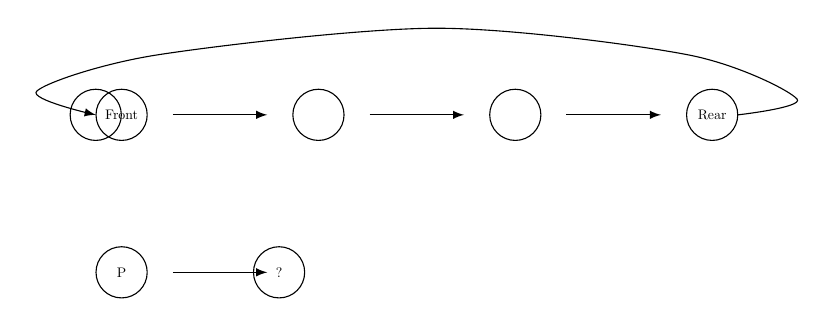
\begin{tikzpicture}[draw, minimum width=1.3cm, minimum height=0.8cm,scale = 0.5]
    \node[draw] (in) at (0,0) {Front};
    \node[draw] (out) at (5,0) {};
    \node[draw] (out) at (10,0) {};
    \node[draw] (out2) at (15,0) {Rear};
    \node[draw] (out) at (0,-4) {P};
    \node at (4,-4) {?};
     \draw[->,>=latex] (1.3,0) -- (3.7,0);
     \draw[->,>=latex] (6.3,0) -- (8.7,0);
     \draw[->,>=latex] (11.3,0) -- (13.7,0);
     \draw[->,>=latex] (1.3,-4) -- (3.7,-4);
  
  \draw [->,>=latex] plot [smooth, tension = 0.5] coordinates { (out2.east) ($(out2.east) + (1.5,0.4)$) 
  ($($($(out2.east) + (1.5,0.6)$)!0.3! (8,2)$) + (0,0.5)$)
  (8,2.2) 
  ($($($(in.west) + (-1.5,0.6)$)!0.3! (8,2)$) + (0,0.5)$)
  ($(in.west) + (-1.5,0.6)$) (in.west) } node {};
  
\end{tikzpicture}

       
       

%https://gateoverflow.in/118378/gate2017-2-36?show=118714#a118714

\usetikzlibrary{trees}

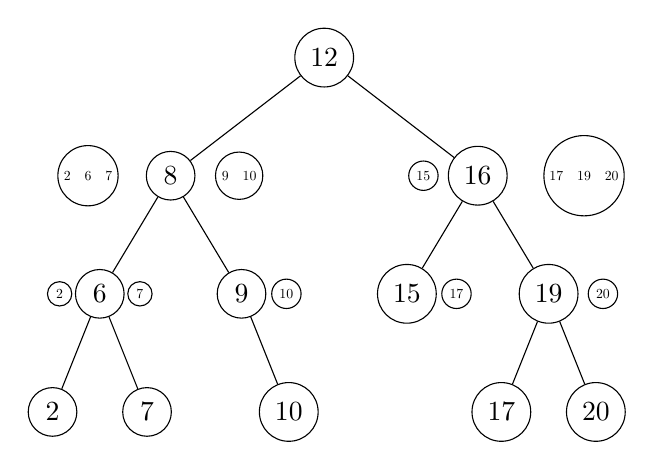
\begin{tikzpicture}[level distance=2.5cm,
level 1/.style={sibling distance=6.5cm},
level 2/.style={sibling distance=3cm},
level 3/.style={sibling distance=2cm},
scale=0.6]
\begin{scope}
\tikzstyle{every node}=[circle,draw]

\node{12}
    child {
    node {8} 
        child {
            node {6}
            child { node {2}}
            child { node {7}}}
        child { node {9}
            child [missing]
            child {node {10}}}
}
child {
 node{16} 
    child {
    node {15}}
    child { node {19}
        child { node {17}}
        child {node{20}}
    }
 }
  ;
\end{scope}

\node at (-5,-2.5){2\quad 6\quad 7 };
\node at (-1.8,-2.5){9\quad 10 };
\node at (2.1,-2.5){15 };
\node at (5.5,-2.5){17\quad 19\quad 20 };
\node at (-5.6,-5){2 };
\node at (-3.9,-5){7 };
\node at (-0.8,-5){10 };
\node at (2.8,-5){17 };
\node at (5.9,-5){20 };
\end{tikzpicture}


%https://gateoverflow.in/118292/gate-cse-2017-set-1-question-12#120564
%https://gateoverflow.in/118292/gate2017-1-12?show=120564#a120564


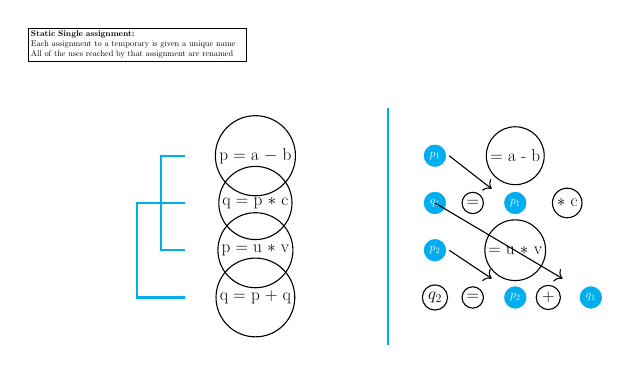
\begin{tikzpicture}[stack/.style={
  rectangle split, rectangle split parts=5, draw, anchor=center},
  myarrow/.style={single arrow, draw=none},scale=0.6,transform shape]

\node [draw,rectangle,align=left,text width=9cm,above] (mid)
  {\textbf{Static Single assignment:} \\ Each assignment to a temporary is given a unique name \\ All of the uses reached by that assignment are renamed};

\node[font= \huge] at (2.5,-2) {p = a $-$ b};
 
\node[font= \huge] at (2.5,-3) {q = p $*$ c};
\node[font= \huge] at (2.5,-4) {p = u $*$ v};
\node[font= \huge] at (2.5,-5) {q = p $+$ q};
\draw[-,color= cyan,thick] (1,-2) -- (0.5,-2) -- (0.5,-4) -- (1,-4);

\draw[-,color= cyan,thick] (1,-3) -- (0,-3) -- (0,-5) -- (1,-5);
\draw[-,color= cyan,thick] (5.3,-1)--(5.3,-6);
\node[font= \huge] at (8,-2) { = a - b};
\node[font=\Large,circle, inner sep=0pt, minimum size=1cm, color=white, fill=cyan] at (6.3,-2){$p_1$};
\node[font=\Large,circle, inner sep=0pt, minimum size=1cm, color=white, fill=cyan] at (8,-3){$p_1$};
\node[font=\Large,circle, inner sep=0pt, minimum size=1cm, color=white, fill=cyan] at (6.3,-3){$q_1$};
\node[font=\Large,circle, inner sep=0pt, minimum size=1cm, color=white, fill=cyan] at (6.3,-4){$p_2$};
\node[font=\Large,circle, inner sep=0pt, minimum size=1cm, color=white, fill=cyan] at (8,-5){$p_2$};
\node[font=\Large,circle, inner sep=0pt, minimum size=1cm, color=white, fill=cyan] at (9.6,-5){$q_1$};
\node[font= \huge] at (7.1,-3) {=};
\node[font= \huge] at (8,-4) { = u $*$ v};
\node[font= \huge] at (7.1,-5) {= };
\node[font= \huge] at (8.7,-5) {$+$};
\node[font= \huge] at (9.1,-3) {$*$ c};
\node[font= \huge] at (6.3,-5) {$q_2$};
\draw[->](6.6,-2)--(7.5,-2.7);
\draw[->](6.3,-3)--(9,-4.6);
\draw[->](6.6,-4)--(7.5,-4.6);

\end{tikzpicture}

%https://gateoverflow.in/313521/gate2017-ec-1-ga-7?show=313839#a313839
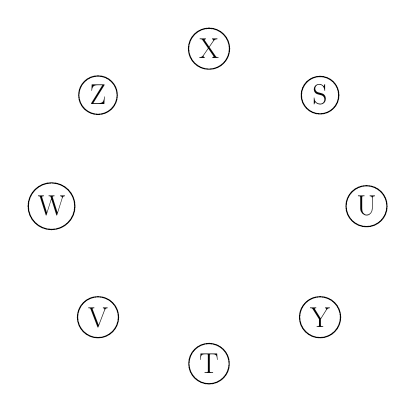
\begin{tikzpicture}[scale=0.5]
\node[font = \huge,draw,circle] at (-4,0) {W} ;
\node[font = \huge,draw,circle] at (4,0) {U} ;
\node[font = \huge,draw,circle] at (0,4) {X} ;
\node[font = \huge,draw,circle] at (0,-4) {T} ;

\node[font = \huge,draw,circle] at (2.82,2.82) {S} ;
\node[font = \huge,draw,circle] at (2.82,-2.82) {Y} ;
\node[font = \huge,draw,circle] at (-2.82,2.82) {Z} ;
\node[font = \huge,draw,circle] at (-2.82,-2.82) {V} ;
\end{tikzpicture}
%%%%%%%%https://gateoverflow.in/313658/gate2017-me-1-ga-3
\usetikzlibrary{arrows}



%\newcommand{\AxisRotator}[1][rotate=0]{%
 %   \tikz [x=0.25cm,y=0.60cm,line width=0.7mm,-stealth,#1] \draw (0,0) arc (-150:150:1 and 1);%
%}

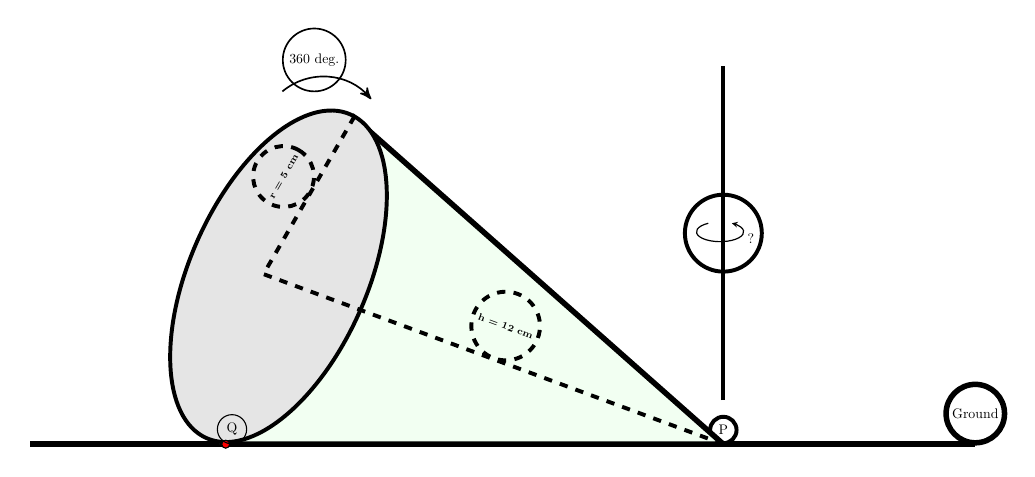
\begin{tikzpicture}[scale=0.8]
\draw[line width = 0.5mm] (10,0.7)node[above] at (10,0) {P}  -- (10,6) node [midway] {\AxisRotator[rotate=-90]?};
\draw[thick,line width=0.7mm] (-1,0) -- (14,0)node [above]{Ground};

\draw [-,line width= 0.7mm,fill=green!5] (2,0)--(10,0) --(4.1,5.22);

\draw[rotate=-24,line width= 0.5mm,fill = black!10 ] (1.6,3.63) ellipse (40pt and 80pt);

\draw [-,line width= 0.5mm,dashed](10,0) -- node [midway,sloped,above,font=\scriptsize]{\textbf{h = 12 cm}} (2.7,2.7) -- node [midway,sloped,above,font=\scriptsize]{\textbf{r = 5 cm}}(4.2,5.3);

 \draw[->,>=stealth',semithick] (3,5.6)node[above=0.4cm, right] {360 deg.} arc (130:40:1cm);
     \draw [fill=red, draw=black] (2.1,0) circle (1.8pt);
 \node[above] at (2.2,0){Q};
\end{tikzpicture}

%%%%%%%%https://gateoverflow.in/313480/gate2017-ce-1-ga-10  
\begin{tikzpicture}

\draw[-] (0,0) -- (0,11);
\draw[-] (-0.2,0.5)node[left]{0} -- (11,0.5);
\draw[-] (-0.2,1.5)node[left]{2} -- (11,1.5);
\draw[-] (-0.2,2.5)node[left]{4}  -- (11,2.5);
\draw[-] (-0.2,3.5) node[left]{6} -- (11,3.5);
\draw[-] (-0.2,4.5)node[left]{8}  -- (11,4.5);
\draw[-] (-0.2,5.5)node[left]{10}  -- (11,5.5);
\draw[-] (-0.2,6.5)node[left]{12}  -- (11,6.5);
\draw[-] (-0.2,7.5)node[left]{14}  -- (11,7.5);
\draw[-] (-0.2,8.5)node[left]{16}  -- (11,8.5);
\draw[-] (-0.2,9.5) node[left]{18} -- (11,9.5);
\draw[-] (-0.2,10.5) node[left]{20} -- (11,10.5);

\draw[-,fill=pink!60] (0.5,0.5) -- (0.5,1.5) -- (1.7,1.5)-- (1.7,0.5) -- cycle;
\draw[-,fill=yellow!60] (0.5,1.5) -- (0.5,5) -- (1.7,5)-- (1.7,1.5) -- cycle;
\draw[-,fill=cyan!60] (0.5,5) -- (0.5,6.5) -- (1.7,6.5)-- (1.7,5) -- cycle;

\draw[-,fill=pink!60] (4.5,0.5) -- (4.5,3) -- (5.7,3)-- (5.7,0.5) -- cycle;
\draw[-,fill=yellow!60] (4.5,3) -- (4.5,7) -- (5.7,7)-- (5.7,3) -- cycle;
\draw[-,fill=cyan!60] (4.5,7) -- (4.5,8) -- (5.7,8)-- (5.7,7) -- cycle;

\draw[-,fill=pink!60] (2.5,0.5) -- (2.5,5.5) -- (3.7,5.5)-- (3.7,0.5) -- cycle;
\draw[-,fill=yellow!60] (2.5,5.5) -- (2.5,6.5) -- (3.7,6.5)-- (3.7,5.5) -- cycle;
\draw[-,fill=cyan!60] (2.5,6.5) -- (2.5,10.5) -- (3.7,10.5)-- (3.7,6.5) -- cycle;

\draw[-,fill=pink!60] (6.5,0.5) -- (6.5,1.5) -- (7.7,1.5)-- (7.7,0.5) -- cycle;
\draw[-,fill=yellow!60] (6.5,1.5) -- (6.5,3) -- (7.7,3)-- (7.7,1.5) -- cycle;
\draw[-,fill=cyan!60] (6.5,3) -- (6.5,4.5) -- (7.7,4.5)-- (7.7,3) -- cycle;

\draw[fill=pink!90,postaction={
        pattern=north west lines
    }] (8.5,0.5) -- (8.5,2.5) -- (9.7,2.5)-- (9.7,0.5) -- cycle;
\draw[-,fill=yellow!60] (8.5,2.5) -- (8.5,7.5) -- (9.7,7.5)-- (9.7,2.5) -- cycle;
\draw[-,fill=cyan!60] (8.5,7.5) -- (8.5,8) -- (9.7,8)-- (9.7,7.5) -- cycle;

\node[below,font=\huge] at (1.1,0.5){$c_1$};
\node[below,font=\huge] at (3.1,0.5){$c_2$};
\node[below,font=\huge] at (5.1,0.5){$c_3$};
\node[below,font=\huge] at (7.1,0.5){$c_4$};
\node[below,font=\huge] at (9.1,0.5){$c_5$};

\filldraw [fill=cyan!60] (9,8.3) rectangle (10.2,8.8)node[right]{bed};
\filldraw [fill=yellow!60, draw=black] (9,8.8) rectangle (10.2,9.3)node[right]{chair};
\filldraw [fill=pink!60, draw=black] (9,9.3) rectangle (10.2,9.8)node[right]{table};
\node at(4.5,-0.5) {Carpenter(C)};
\node[rotate=90] at(-1,4.5) {number of furniture Items};

\end{tikzpicture}

\begin{tikzpicture}
\begin{axis}[
    ybar stacked,
	bar width=25pt,
	ytick={0,2,4,6,8,10,12,14,16,18,20},
	grid = both,
	        ymajorgrids=true,
	        xmajorgrids = false,
	        xtick = \empty,
    %minor tick num=3
    %grid style={line width=.1pt, draw=gray!10},
   % enlargelimits=0.15,
    %legend style={at={(0.5,-0.20)},
     % anchor=north,legend columns=-1},
      % legend style={
    %  anchor=north},
    ylabel={Number of furniture items},
    xlabel={Carpenter(C)},
    symbolic x coords={C1, C2, C3, C4, C5},
    xtick=data,
    reverse legend
    ]
   
\addplot+[ybar,fill=pink,postaction={
        pattern=north west lines
    },draw=black] plot coordinates {(C1,2) (C2,10) (C3,5) (C4,2) (C5,4)
  };
\addplot+[ybar,fill=yellow,postaction={ pattern=north east lines}] plot coordinates {(C1,7) (C2,2) (C3,8) (C4,3) (C5,10)};
\addplot+[ybar,fill=cyan,postaction={
        pattern=crosshatch dots
    },draw=black] plot coordinates {(C1,3) (C2,8) (C3,2) (C4,3) (C5,1)};

%\legend{\strut Bed, \strut Table, \strut Chair}
\legend{ Chair,  Table, Bed}

\end{axis}
\end{tikzpicture}


%https://gateoverflow.in/118286/gate2017-1-6?show=208895#a208895
% first diagram
\begin{tikzpicture}[iv/.style={circle,draw,minimum size = 8pt,inner
sep=1pt},emph/.style={edge from parent/.style={densely dashed,draw}},level 1/.style={sibling distance=24mm},level 2/.style={sibling distance=22mm},level 3/.style={sibling distance=20mm}, scale = 0.4]
\node[iv]{}
    child[missing]
    child {node[iv]{}
          child[missing]
          child[] {node[iv]{}
                child[missing]
                child[emph]{node[iv]{}}}};

\end{tikzpicture}


%https://gateoverflow.in/118286/gate2017-1-6?show=208895#a208895
% second diagram
\begin{tikzpicture}[every node/.style={circle,draw,minimum size = 10pt,inner sep=1pt},level 1/.style={sibling distance=80mm},level 2/.style={sibling distance=40mm},level 3/.style={sibling distance=25mm}, scale = 0.4]
\node{}
    child {node{}
          child {node{}
                child {node{}}
                child {node{}}}
          child {node{}
                child {node{}}
                child {node{}}}}
    child {node{}
          child {node{}
                child {node{}}
                child {node{}}}
          child {node{}
                child {node{}}
                child {node{}}}};

\end{tikzpicture}

%%%%%%%%%%%https://gateoverflow.in/118395/gate2017-2-50?show=123981#a123981

\usetikzlibrary{shapes}

\begin{tikzpicture}[scale=0.5,transform shape, iv/.style={draw,circle,thick,minimum size=50pt,inner
sep=3pt,text=black},ev/.style={draw,rectangle,minimum
size=30pt,inner sep=3pt,text=black},scale = 1, auto,level distance=2.5cm,level 1/.style={sibling distance=40mm},level 2/.style={sibling distance=30mm},level 3/.style={sibling distance=25mm},font=\Huge]


\node[iv] at (-2,-7)  {0.41}
  child {node[ev]{0.19 } node[below,yshift=-0.5cm]{S}}
  child {node[ev]{0.22}node[below,yshift=-0.5cm]{P}};

    \draw [-,dashed] (1.5,-6) -- (1.5,-13);
   
    \node[iv] at (6,-7)  {0.59}
  child {node[iv]{0.25 }
  child{node[ev]{0.08}node[below,yshift=-0.5cm]{T}}
  child{node[ev]{0.17}node[below,yshift=-0.5cm]{R}}}
  child {node[ev]{0.34}node[below,yshift=-0.5cm]{Q}};

  
  %%
   \node[iv] at (6,-15){1}
  child {node[iv] at (-1,0) {0.41} 
  child{node [ev]{0.19} node[below,yshift=-0.5cm]{S}
  edge from parent node [left,yshift=0.2cm]{0}
  }
   %edge from parent[left]node []{0}
  child{node[ev]{0.22}  node[below,yshift=-0.5cm]{P}
  edge from parent node [right,yshift=0.2cm]{1}
  }
  edge from parent node [left,yshift=0.2cm]{0}
  }
  child{node[iv] at (1,0){0.59}
  child{node[iv]{0.25}
  child{node [ev]{0.08} node[below,yshift=-0.5cm]{T}edge from parent node[left,yshift=0.2cm]{0}}
  child{node[ev]{0.17} node[below,yshift=-0.5cm]{R}edge from parent node[right,yshift=0.2cm]{1}}
  edge from parent node[left,yshift=0.2cm]{0}
  }
  child{node[ev]{0.34} node[below,yshift=-0.5cm]{Q}edge from parent node[right,yshift=0.2cm]{1}}
  edge from parent node[right,yshift=0.2cm]{1}
  };

\node[font = \huge] at (0,0) {P: 0.22};
\node[font = \huge] at (3,0) {Q: 0.34};
\node[font = \huge] at (6,0)(r) {R: 0.17};
\node[font = \huge] at (9,0) {S: 0.19};
\node[font = \huge] at (12,0)(t) {T: 0.08};

\node[font = \huge] at (1.5,-2)(p) {P: 0.22};
\node[font = \huge] at (4,-2) {Q: 0.34};
\node[font = \huge] at (6.5,-2) (s){S: 0.19};
\node[font = \huge] at (8.5,-2)(1) { 0.25};

\draw [-] (r) -- (1) -- (t);

\node[font = \huge] at (1.5,-5)(2) { 0.41};
\node[font = \huge] at (4,-5) {0.25};
\node[font = \huge] at (6.5,-5)(1) { Q:0.34};
\draw[-] (p) -- (2) -- (s);

\node [font = \huge,text width=1.5cm] at (-3,-18){P:01 \\ Q:11 \\R:101\\S:00\\T:100};
% \node [font = \huge] at (-3,-13){Q:11};
% \node [font = \huge] at (-3,-13.5){R:101};
% \node [font = \huge] at (-3,-14){S:00};
% \node [font = \huge] at (-3,-14.5){T:100};

%\node [font = \huge] at (-3,-13){Q};
%\node [font = \huge] at (-3,-13.5){R};
%\node [font = \huge] at (-3,-14){S};
%\node [font = \huge] at (-3,-14.5){T};




\end{tikzpicture}



%%%%%%%%%%%https://gateoverflow.in/118395/gate2017-2-50?show=123981#a123981

\usetikzlibrary{shapes}

\begin{tikzpicture}[iv/.style={draw,fill=red!50,circle,minimum size=40pt,inner
sep=0pt,text=black},ev/.style={draw,fill=yellow,rectangle,minimum
size=40pt,inner sep=0pt,text=black},scale = 1, auto]


\node[iv] at (-2,-7)  {0.41}
  child {node[ev]{0.19 }}
  child {node[ev]{0.22}};
  \node at (-2.7,-9.2) {S};
    \node at (-1.6,-9.2) {P};
    \draw [-,dashed] (1.5,-6) -- (1.5,-10);
   
    \node[iv] at (6,-7)  {0.59}
  child {node[iv]{0.25 }
  child{node[ev]{0.08}}
  child{node[ev]{0.17}}}
  child {node[ev]{0.34}};
  \node at (6.5,-9.2) {Q};
   \node at (4.5,-10.7) {T};
    \node at (6,-10.7) {R};
  
  %%
   \node[iv] at (6,-12.5){1}
  child {node[iv] at (-1,0){0.41}
  child{node [ev]{0.19}}
  child{node[ev]{0.22}}}
  child{node[iv] at (1,0){0.59}
  child{node[iv]{0.25}
  child{node [ev]{0.08}}
  child{node[ev]{0.17}} }
  child{node[ev]{0.34}}};

 \node at (4.7,-13.3) {0};
   \node at (7.2,-13.3) {1};
    \node at (3.7,-14.5) {0};
      \node at (4.9,-14.5) {1};
      
       \node at (7.2,-14.5) {0};
      \node at (8.3,-14.5) {1};
      
       \node at (6.3,-16.3) {0};
      \node at (7.7,-16.3) {1};
      
       \node at (3.5,-16.2) {S};
      \node at (5,-16.2) {P};
       \node at (8.6,-16.2) {Q};
      \node at (7.7,-17.7) {R};
       \node at (6.3,-17.7) {T};
      

  
  
\node[font = \huge] at (0,0) {P: 0.22};
\node[font = \huge] at (3,0) {Q: 0.34};
\node[font = \huge] at (6,0)(r) {R: 0.17};
\node[font = \huge] at (9,0) {S: 0.19};
\node[font = \huge] at (12,0)(t) {T: 0.08};

\node[font = \huge] at (1.5,-2)(p) {P: 0.22};
\node[font = \huge] at (4,-2) {Q: 0.34};
\node[font = \huge] at (6.5,-2) (s){S: 0.19};
\node[font = \huge] at (8.5,-2)(1) { 0.25};

\draw [-] (r) -- (1) -- (t);

\node[font = \huge] at (1.5,-5)(2) { 0.41};
\node[font = \huge] at (4,-5) {0.25};
\node[font = \huge] at (6.5,-5)(1) { Q:0.34};
\draw[-] (p) -- (2) -- (s);

\node [font = \huge] at (-3,-12.5){P:01};
\node [font = \huge] at (-3,-13){Q:11};
\node [font = \huge] at (-3,-13.5){R:101};
\node [font = \huge] at (-3,-14){S:00};
\node [font = \huge] at (-3,-14.5){T:100};

%\node [font = \huge] at (-3,-13){Q};
%\node [font = \huge] at (-3,-13.5){R};
%\node [font = \huge] at (-3,-14){S};
%\node [font = \huge] at (-3,-14.5){T};




\end{tikzpicture}

%%%%%%%%%%%%%%%%https://gateoverflow.in/118331/gate2017-1-48?show=119365#a119365

%\usetikzlibrary{calc,shapes.multipart,chains,arrows}


\begin{tikzpicture}[transform shape,scale = .5,font=\Large]
\node[draw,ellipse,text=red] at (0,0){\bf{.}};
\node[draw,circle,fill=red,minimum size=0.2cm,inner sep=0]{};
\node[draw,circle,text=red] at (3,0){\bf{.}};
\node[draw,circle,fill=red,minimum size=0.2cm,inner sep=0]at (3,0){};
\node[draw,circle,text=red] at (6,0){\bf{.}};
\node[draw,circle,fill=red,minimum size=0.2cm,inner sep=0]at (6,0){};
\draw[|-|,line width = 0.5mm](-3,0) -- (8,0);
\node[above,color=red] at (-0.4,0.2) {miss};
\node[above] at (3.6,0.2) {hit};

\draw[->,line width = 0.5mm,color=cyan] (7,3) node [above, font = \small,color=black] {neighbourhood of probe} -- (6.2,0.3);

%\draw[->,line width = 0.5mm] (1.3,2) node [above, font = \small] {1st probe} -- (2.8,0.3);
\draw[bend left =45,->,line width = 0.5mm ,color=cyan](1,2)node [above,color=black,yshift=0.2cm]{1st probe} to  (6,0.2);
\node[yshift = -0.4cm,,xshift=0cm,right,color = red] at (6.4,0.2) {miss};
\draw[bend left =90,->,line width = 0.5mm,color=cyan ](0,0) to node [above,color=black]{3rd probe} (3,0.2);

\draw[bend left =95,->,line width = 0.5mm,color=cyan ](6,0) to node [below,color=black]{2nd probe} (0,-0.2);

  
\end{tikzpicture}

%https://gateoverflow.in/118305/gate2017-1-25#119604
\tikzstyle{decision} = [diamond, draw, fill=blue!20, 
    text width=4.5em, text badly centered, node distance=3cm, inner sep=0pt]
\tikzstyle{block} = [rectangle, draw, fill=blue!20, 
    text width=5em, text centered, rounded corners, minimum height=4em]
\tikzstyle{line} = [draw, -latex']
\tikzstyle{cloud} = [draw, ellipse,fill=red!20, node distance=3cm,
    minimum height=2em]
    
\begin{tikzpicture}[node distance = 2cm, auto]
    % Place nodes
    \node [block] (L1) {L1};
    \node [block, left of= L1, above of = L1] (cpu) {CPU};
  
    \node [block, below of=L1] (L2) {L2};
   \node (r4) [right of = L1,above of = L2,node distance=1cm,text width=2cm] { 140 mem ref};
   \node (r5) [below of = L1,,node distance=4cm,text width=2cm] {};
\node (A) at (1.2,-3) {7 mem ref miss};
\node (B) at (1.2,-4.5) {L2 miss rate = $\frac{7}{140}$ = 0.05};
\node (C) at (1.9,2) {1400 memory references };
\node (D) at (-.3,3.5) {1000 Instructions};
    % Draw edges
   \path [line] (L1) -- (L2);
   \path [line] (L2) -- (r5);
    \path [line] (cpu) -| (L1);
    \draw[] (L1.east) node[right] {Miss Rate = 0.1} (L2.north); 
   %  \draw[] (L1.south) node[right] {Miss Rate = 0.1} (L2.east
  
\end{tikzpicture}


%https://gateoverflow.in/118410/gate2017-1-ga-7?show=120331#a120331
%case 1
          \begin{tikzpicture}[node distance=2cm,auto,>=Latex]
          
             \tikzstyle{nodep}=[circle,scale=1,text=white,draw= blue!80,fill=blue!30]
             \node [circle,draw= cyan!80,fill= cyan!25,scale= 8] (a) at (0,0) { }; 
             \node[nodep] (b) [above of = a] {M};
              \node[nodep] (c) [above left of = a] {M};
              \node[nodep] (d) [left of = a,label={[green] left:{\checkmark}}] {W};
              \node[nodep] (e) [below left of = a,label={[green] below left:{\checkmark}}] {W};
              \node[nodep] (f) [below of = a,label={[green] below:{\checkmark}}] {W};
              \node [rectangle,minimum height=.6cm,minimum width=.6cm,text=white,draw= blue!80,fill=blue!30] (g) [below right of = a,label={[red] below right:{\ding{55}}}] { };
              \draw[->] (d) to [bend right=90, looseness=2] (e);
              \draw[->] (e) to [bend right=90, looseness=2] (f);
              \draw[->] (f) to [bend right=90, looseness=2] (g);
              \draw[->] (2,-.2) -- (1.5,-1);
              
          \end{tikzpicture}
          
 %case 2         
           \begin{tikzpicture}[node distance=2cm,auto,>=Latex]
          
             \tikzstyle{nodep}=[circle,scale=1,text=white,draw= blue!80,fill=blue!30]
             \node [circle,draw= cyan!80,fill= cyan!25,scale= 8] (a) at (0,0) { }; 
             \node[nodep] (b) [above of = a,xshift=-.8cm,yshift= -.2cm] {M};
              \node[nodep] (c) [above right of = a,xshift=-.6cm,yshift= .4cm] {M};
              \node [nodep] (g) [right  of = a,label={below right:{Right Handed Man}}] {M};
               \node[nodep] (d) [left of = a,label={[green] left:{\checkmark}}] {W};
               \node[nodep] (f) [below of = a,xshift=.8cm,yshift= .2cm,label={[green] below right:{\checkmark}}] {M};
              \node[nodep] (e) [below left of = a,xshift=.7cm,yshift= -.4cm,label={[green] 240:{\checkmark}}] {W};
              \draw[->] (d) to [bend right=90, looseness=2] (e);
              \draw[->] (e) to [bend right=90, looseness=2] (f);
             \node (h) at (3.5,-3) {Left handed Man};
              \draw[->] (h) -- (f);
              
          \end{tikzpicture}
         

            
%https://gateoverflow.in/118701/gate2017-1-02?show=123153#a123153

            \begin{tikzpicture}
                \coordinate [label={left:{\tiny $\exists x \forall y$}}] (H) at (-1,1); 
                \coordinate [label={right:{\tiny $\exists y \forall x$}}] (C) at (1,1); 
                \coordinate [label={left:{\tiny $\forall y \exists x$}}] (G) at (-1,-1); 
                \coordinate [label={right:{\tiny $\forall x \exists y$}}] (D) at (1,-1); 
                \coordinate [label={left:{\tiny $\forall x \forall y$}}] (A) at (-.5,1.5); 
                \coordinate [label={right:{\tiny $\forall y \forall x$}}] (B) at (.5,1.5); 
                \coordinate [label={left:{\tiny $\exists x \exists y$}}] (F) at (-.5,-1.5); 
                \coordinate [label={right:{\tiny $\exists y \exists x$}}] (E) at (.5,-1.5); 
                \coordinate [label={center:{\tiny $P(x,y)$}}] (P) at (0,0); 
                \draw[Latex-Latex] (A)--(B);
                \draw[-Latex] (B)--(C);
                \draw[-Latex] (C)--(D);
                \draw[-Latex] (D)--(E);
                \draw[-Latex] (A)--(H);
                \draw[-Latex] (H)--(G);
                \draw[-Latex] (G)--(F);
                \draw[Latex-Latex] (F)--(E);
                
            \end{tikzpicture}
            
            
            %https://gateoverflow.in/313487/gate2017-ce-1-ga-3?show=313973#a313973
            \def\firstcircle{(0,0) circle (1.5cm)}
 \def\secondcircle{(0:2cm) circle (1.5cm)}

  \colorlet{circle edge}{blue!50}
  \colorlet{circle area}{blue!20}

  \tikzset{filled/.style={fill=circle area, draw=circle edge, thick}, outline/.style={draw=circle edge, thick}}

  \setlength{\parskip}{5mm}

\centering
% Set A and B

 \begin{tikzpicture}
  \begin{scope}
    \clip \secondcircle;
    \draw[filled, even odd rule] \firstcircle
                                 \secondcircle node {Lamp};
  \end{scope}
     \draw[outline] \firstcircle node {Bulb}
               \secondcircle;
   \end{tikzpicture}
   
   
   %%%%%%%%%%%%%%%%%%%%%%%%%%%%%%%
   
 

\usetikzlibrary{decorations.text,calc,arrows.meta}

\begin{tikzpicture}
\coordinate (O) at (0,0);


\draw (O) circle (1.5);
\draw (O) circle (1);


\draw[decoration={text along path,reverse path,text align={align=center},text={Bench}},decorate] (1.6,-1) arc (0:180:1.6);
\draw[decoration={text along path,reverse path,text align={align=center},text={Bed}},decorate] (2.6,-1.5) arc (0:180:2.6);



\end{tikzpicture}


  
  %%https://gateoverflow.in/313523/gate2017-ec-1-ga-5?show=313869#a313869

  \usetikzlibrary{decorations.text,calc,arrows.meta}

\begin{tikzpicture}
\coordinate (O) at (0,0);
\coordinate (O) at (0,0);
\coordinate (O1) at (-1.6,0);

\coordinate (O2) at (-3,0);

\draw (O) circle (1.3);
\draw (O) circle (0.9);
\draw (O1) circle (1);
\draw (O2) circle (0.7);

\draw[decoration={text along path,reverse path,text align={align=center},text={C}},decorate] (1.6,-1.5) arc (0:180:1.6);
\draw[decoration={text along path,reverse path,text align={align=center},text={B}},decorate] (2.6,-1.65) arc (0:180:2.6);
\node at (-1.6,0.7){S};
\node at (-3,0.3){T};

\node at (-1,-2.6)[text width=2cm,align=left]{T = Tables\\S = Shelves\\B = Benches\\C = Chairs};
%\node at (0,-2.5){S = shelves};
%\node at (0,-3){B = benches};
%\node at (0,-3.5){C = Chairs};





\end{tikzpicture}

%https://gateoverflow.in/313508/gate2017-ec-2-ga-4?show=313929#a313929
%Subarna
\begin{tikzpicture}[>=stealth]
 \begin{scope}[ decoration={
    markings,
    mark=at position 0.65 with {\arrow{>}}}
    ] 
    \draw[postaction={decorate}] (2.1,1.02) node[below,xshift=1pt, yshift=1pt, scale=0.8] {\tiny P} -- node[xshift=-4pt, scale=0.8]{\tiny $3$}(2.1,1.6) node[yshift=2pt, xshift=-1pt, scale=0.8] {\tiny X};
    \draw[postaction={decorate}] (2.1,1.6) -- node[yshift=4pt, scale=0.8] {\tiny $4$}(3,1.6) node[below,xshift=2pt, yshift=6pt, scale=0.8] {\tiny Q};
    \draw[postaction={decorate}](3,1.6) -- node[xshift=2pt,yshift= -4pt,rotate= 25, scale=0.6, blue] {\tiny $\sqrt{4^{2} + 3^{2}} = 5$} (2.1,1);
    \draw[postaction={decorate}] (2.1,1) -- node[xshift = 6pt,rotate=17,scale=0.8] {\tiny $10$}(0,-0.1);
    \draw[postaction={decorate}] node[xshift=-4pt,scale=0.8]{\tiny Y}(0,-0.1) -- node[xshift=-4pt,scale=0.8] {\tiny $6$}(0,1) node[xshift=-2pt,yshift=2pt, scale=0.8]{\tiny Z};
    \draw[postaction={decorate}] (0,1) -- node[yshift=4pt,scale=0.8,thick] {\tiny $?$}(2,1);
    
    \draw[|<->|] (0.1,-0.5) -- node[below,rotate=19, scale=0.8] {\tiny $15$} (3.2,1.1);
    
    \draw (2.5,-0.05)node[xshift=-3pt, scale=0.8] {\tiny W} -- (3.5,-0.05)node[xshift=3pt, scale=0.8] {\tiny E};
    \draw (3,0.5)node[yshift=3pt, scale=0.8] {\tiny N} -- (3,-0.5)node[yshift=-3pt, scale=0.8] {\tiny S};
 \end{scope}
\end{tikzpicture}


%%%%%%%%%%%%%
%https://gateoverflow.in/313508/gate2017-ec-2-ga-4?show=313929#a313929

\thispagestyle{empty}

\usetikzlibrary{arrows}
%\newcommand{\midarrow}{\tikz \draw[-triangle 90] (0,0) -- +(.1,0);}


\begin{tikzpicture}[scale=0.5]
\begin{scope}[very thick, every node/.style={sloped,allow upside down}]
  \draw (9,4.5)-- node {\midarrow} (6,3) -- node {\midarrow} (0,0);
   \draw[|<->|] (0.5,-1.2)-- node[below] {15} (9.5,3.3);
 \draw (0,0)-- node {\midarrow} (0,3);
  \draw (0,3)-- node {\midarrow} (6,3);
  \draw (6,3)-- node {\midarrow} (6,4.5);
    \draw (6,4.5)-- node {\midarrow} (9,4.5);
    
    \node[left] at (0,0) {$\textbf{Y}$};
      \node[below] at (6,3) {$\textbf{P}$};
        \node[right] at (9,4.5) {$\textbf{Q}$};
          \node[above] at (6,4.5) {$\textbf{X}$};
           \node[above] at (0,3) {$\textbf{Z}$};
           
           \node[left] at (-.2,1.5){6};
           \node[left] at (5.8,3.8){3};
           \node[above] at (7.5,4.7){4};
            \node[above] at (3,3.2){?};
           \node[below] at (3,1.3){10};
             \node[below,rotate=25] at (7.5,3.8){\tiny $\sqrt{3^2 + 4^2}=5$};
             
           
\end{scope}
  \draw[-,thick] (9,-6) -- (9,-2);
             \draw[-,thick] (7,-4) -- (11,-4);
             \node[below] at (9,-6){$\bf{S}$};
               \node[left] at (7,-4){$\bf{W}$};
                 \node[right] at (11,-4){$\bf{E}$};
                   \node[above] at (9,-2){$\bf{N}$};
\end{tikzpicture}



  %https://gateoverflow.in/118423/gate2017-2-ga-9    
  \begin{tikzpicture}[scale=1.5]
      \draw[->] (-1.5,0) -- (1.2,0) node[right] {$x$};
     % \draw[->] (0,-1) -- (0,1.5) node[above] {$y$};
      \filldraw (-0.24,0) circle[radius=1pt];
      \draw[-,dotted,thick] (-0.24,-0.63) -- (-0.24,0) node[above] {$k$};
      \draw[scale=0.5,domain=-2.5:1.2,smooth,variable=\x,blue]
      plot (\x,{(exp(\x))+0.5*pow(\x,2)-2});% node [below] {f};
      \node at (0,-1) {Plot of $f(x)$};
    \end{tikzpicture}
    
     %https://gateoverflow.in/118423/gate2017-2-ga-9    
  \begin{tikzpicture}[scale=1.5]
      \draw[->] (-1.5,0) -- (1.2,0) node[right] {$x$};
      %\draw[->] (0,-1) -- (0,1.5) node[above] {$y$};
       \filldraw (-0.24,0) circle[radius=1pt];
      \draw[-,dotted,thick] (-0.24,-0.63) -- (-0.24,0) node[above] {$k$};
      \filldraw (-1.3,0) circle[radius=1pt];
       \node at (-1.3,0)[below] {-5};
        \filldraw (1,0) circle[radius=1pt];
       \node at (1,0)[below] {5};
      \draw[scale=0.5,domain=-2.5:1.2,smooth,variable=\x,blue]
      plot (\x,{(exp(\x))+0.5*pow(\x,2)-2});% node [below] {f};
      \node at (0,-1) {Image 1};
    \end{tikzpicture}
    
     %https://gateoverflow.in/118423/gate2017-2-ga-9    
  \begin{tikzpicture}[scale=1.5]
      \draw[->] (-1.5,0) -- (1,0) node[right] {$x$};
     % \draw[->] (0,-1) -- (0,1.5) node[above] {$y$};
       \filldraw (-0.24,0) circle[radius=1pt];
      \draw[-,dotted,thick] (-0.24,-0.63) -- (-0.24,0) node[above] {$k$};
      \filldraw (-0.8,0) circle[radius=1pt];
       \node at (-0.8,0)[below] {-5};
        \filldraw (0.8,0) circle[radius=1pt];
       \node at (0.8,0)[below] {5};
      \draw[scale=0.5,domain=-2.5:1.2,smooth,variable=\x,blue]
      plot (\x,{(exp(\x))+0.5*pow(\x,2)-2});% node [below] {f};
      \node at (0,-1) {Image 2};
    \end{tikzpicture}
    
     %https://gateoverflow.in/118423/gate2017-2-ga-9    
  \begin{tikzpicture}[scale=1.5]
      \draw[->] (-1.5,0) -- (1,0) node[right] {$x$};
     % \draw[->] (0,-1) -- (0,1.5) node[above] {$y$};
       \filldraw (-0.24,0) circle[radius=1pt];
      \draw[-,dotted,thick] (-0.24,-0.63) -- (-0.24,0) node[above] {$k$};
      \filldraw (-1.2,0) circle[radius=1pt];
       \node at (-1.2,0)[below] {-5};
        \filldraw (0.2,0) circle[radius=1pt];
       \node at (0.2,0)[below] {5};
      \draw[scale=0.5,domain=-2.5:1.2,smooth,variable=\x,blue]
      plot (\x,{(exp(\x))+0.5*pow(\x,2)-2});% node [below] {f};
      \node at (0,-1) {Image 3};
    \end{tikzpicture}
% \usetikzlibrary{plotmarks}


% \begin{tikzpicture}[dot/.style={draw,rectangle,minimum size=4mm,inner sep=0pt,outer sep=0pt,thick},scale=0.7]
%   \tkzInit[xmax=15,ymax=11,xmin=0,ymin=0]
%   \tkzGrid
%  %  \tkzAxeY
 
%  \foreach \x/\xtext in {0/0,1/2, 2/4, 3/6, 4/8, 5/10,6/12,7/14, 8/16, 9/18, 10/20, 11/22, 12/24, 13/26,14/28,15/30}
% {\draw (\x cm,1pt ) -- (\x cm,-1pt ) node[anchor=north] {$\xtext$};}



% \draw [black] plot [only marks, mark=square] coordinates {(0,0) (1,.3) (2,.6)(3,0.9)(4,1.5)(5,3)(6,4.5)(7,6)(8,6.7)(9,7.1)(10,7.5)(11,7.7)(12,7.9)(13,8)(14,8)(15,8)(2,10)};

% \draw[-] (0,0) -- (1,.3)--(2,.6) -- (3,0.9) -- (4,1.5)-- (5,3)--(6,4.5)--(7,6)--(8,6.7)--(9,7.1)--(10,7.5)--(11,7.7)--(12,7.9)--(13,8)--(14,8)--(15,8);


% \foreach \point in {(0,1.5),(1,1.8),(2,1.9),(3,2.1),(4,2.5),(5,3),(6,4),(7,6),(8,8),(9,9),(10,9.5),(11,10),(12,10.2),(13,10.4),(14,10.4),(15,10.4),(2,9)}{% points
%       \draw[color=red] \point circle (3pt);
% }
% \draw[-] (0,1.5)--(1,1.8)--(2,1.9)--(3,2)--(4,2.5)--(5,3)--(6,4)--(7,6)--(8,8)--(9,9)--(10,9.5)--(11,10)--(12,10.2)--(13,10.4)--(14,10.4)--(15,10.4);

% \node[font = \huge] at (8,-1.5) {Day of the Month};
% \node[font = \huge,rotate= 90] at (-1.5,5) {Pollutant Concentration(ppm)};

% \node[] at (3.5,10){Winter};
% \node[] at (3.5,9.5){Summer};

% \draw (1,10.5) -- (5,10.5) -- (5,8.5) -- (1,8.5) -- cycle;


% \end{tikzpicture}

%https://gateoverflow.in/118301/gate2017-1-21

\begin{karnaugh-map}[4][4][1][][]
        \minterms{4,12,14}
       
      
            \terms{1,3,9,11,6}{X}
        \node at (-0.25,4.7) {ba};           % row name
        \node at (-0.6,4.15) {dc};            % column name
        \draw[ultra thin] (0,4) -- (-1,4.75);  % diagonal line
    \end{karnaugh-map}
    
  %https://gateoverflow.in/118370/gate2017-2-28
\begin{karnaugh-map}[4][4][1][][]
        \minterms{0,4,8,2,10,13,12}
        \maxterms{1,3,7,6,11}
        \implicant{7}{14}
        \implicantedge{1}{3}{9}{11}
       
      
            \terms{5,9,14,15}{d}
        \node at (-0.25,4.7) {WX};           % row name
        \node at (-0.6,4.15) {YZ};            % column name
        \draw[ultra thin] (0,4) -- (-1,4.75);  % diagonal line
    \end{karnaugh-map}
    %
         \usetikzlibrary{positioning}
\tikzset{
  gray box/.style={
    fill=white!20,
    draw=black,
    minimum width={0.5*#1ex},
    minimum height={4em},
  },
  annotation/.style={
    anchor=north,
  }
}

\begin{tikzpicture}[node distance=-0.5pt,font=\Large]
  \node [gray box=2] (p1) {\(P_1\)};

  \node [gray box=3, right=of p1] (p2) {\(P_4\)};
  \node [gray box=28, right=of p2] (p3) {\(P_2\)};
   \node [gray box=7, right=of p3] (p4) {\(P_4\)};
    \node [gray box=9, right=of p4] (p5) {\(P_1\)};
  \node [gray box=2, right=of p5] (p6) {\(P_3\)};
   \node [gray box=16, right=of p6] (p7) {\(P_5\)};
  

 \node [annotation] at (p1.south west) {0};
  \node [annotation] at (p1.south east) {2};
 \node [annotation] at (p2.south east) {5};
  \node [annotation] at (p3.south east) {33};
   \node [annotation] at (p4.south east) {40};
   \node [annotation] at (p5.south east) {49};
  \node [annotation] at (p6.south east) {51};
   \node [annotation] at (p7.south east) {67};
 
\end{tikzpicture}

%https://gateoverflow.in/118304/gate2017-1-24?show=118840#a118840
\begin{tikzpicture}[node distance=-0.5pt]
  \node [gray box=3] (p1) {\(P_1\)};
  \node [gray box=3, right=of p1] (p2) {\(P_2\)};
  \node [gray box=2, right=of p2] (p3) {\(P_4\)};
   \node [gray box=4, right=of p3] (p4) {\(P_1\)};
    \node [gray box=5, right=of p4] (p5) {\(P_3\)};
  

 \node [annotation] at (p1.south west) {0};
  \node [annotation] at (p1.south east) {3};
 \node [annotation] at (p2.south east) {6};
  \node [annotation] at (p3.south east) {8};
   \node [annotation] at (p4.south east) {12};
   \node [annotation] at (p5.south east) {17};
 
 
\end{tikzpicture}

%https://gateoverflow.in/118160/gate-cse-2017-set-2-question-25#118586
%https://gateoverflow.in/118160/gate2017-2-25#118586
\begin{tikzpicture}[>=stealth',shorten >=1pt,auto,node distance=1.5cm]
  \node[state,initial, initial text=]     (1)   {1};
  \node[state] (2)           [right of= 1] {2};
  \node[state] (3)           [right of= 2] {3};
  \node[state] (4)           [above right of= 3] {4};
  \node[state] (5)           [right of= 4] {5};
  \node[state] (6)           [right of= 5] {6};
  \node[state,accepting] (7)           [right of= 6] {7};
  \node[state] (8)           [below right of= 3] {8};
  
  \path[->]
  (1) edge                      node {a,b} (2)
  (2) edge                      node {a,b} (3)
  (3) edge                      node {a}  (4)
      edge                      node {b} (8)
  (4) edge                      node {a,b} (5)
  (5) edge                      node {a,b} (6)
  (6) edge                      node {a,b} (7)
  (7) edge [loop above]         node {a,b} ()
  (8) edge [loop right]         node {a,b} ();
  
\end{tikzpicture}
%https://gateoverflow.in/118302/gate-cse-2017-set-1-question-22#118855
\begin{tikzpicture}[>=stealth',shorten >=1pt,auto,node distance=2cm]
  \node[state]     (A)   {A};
  \node[state] (B) [right of=A] {B};
  \node[state,accepting] (C) [right of=B] {C};
   
   \path[->]
   (A) edge [loop above]         node {a,b} ()
       edge                      node {b} (B)
   (B) edge                      node {a,b} (C);
     
\end{tikzpicture}

%https://gateoverflow.in/118384/gate2017-2-39?show=118678#a118678
\begin{tikzpicture}[>=stealth',shorten >=1pt,node distance=4cm,on grid,auto]
   \node[state,initial,accepting,initial text=] (q_0)     {$q_0$};
   \node[state] (q_2) [right of = q_0] {$q_2$};
   \node[state] (q_3) [below right of = q_2] {$q_3$};
   \node[state] (q_1) [below left of = q_2] {$q_1$};
   
   \path[->]
   (q_0) edge [loop above]      node {b} ()
         edge [bend left=20]    node {null} (q_2)
         edge                   node {a} (q_1)
   (q_1) edge                   node {null,a} (q_2)
         edge                   node {b} (q_3)
   (q_2) edge                   node {null} (q_0)
   (q_3) edge                   node {b} (q_2);
         
\end{tikzpicture}




%https://gateoverflow.in/118278/gate2017-2-21
\begin{tikzpicture}
\tikzstyle{every node}=[circle,draw,scale=0.5]     

\node [label={$\mathbf{e}$}] (a) at (0,1) {};
\node [label=left:{$\mathbf{c}$}](b) at (-1,0) {};
\node [label=right:{$\mathbf{d}$}](c) at (1,-0.5) {};
\node [label=left:{$\mathbf{b}$}](d) at (-1,-1.5) {};
\node [label=below:{$\mathbf{a}$}](f) at (0.2,-2.5) {};


\draw[->,>=stealth',thick] (b) -- (a);
\draw[->,>=stealth',thick] (c) -- (a);
\draw[->,>=stealth',thick] (d) -- (b);
\draw[->,>=stealth',thick] (f) -- (d);
\draw[->,>=stealth',thick] (f) -- (c);



\end{tikzpicture} 

%https://gateoverflow.in/118196/gate-cse-2017-set-2-question-15

\begin{tikzpicture}[scale = 1,font = \sffamily, transform shape, main/.style = {draw, circle}, node distance=2cm and 4cm]
\node[main] (1) {M};
\node[main] (2) [right of=1] {N};
\node[main] (3) [right of=2] {O};
\node[main] (4) [below of=1] {R};
\node[main] (5) [right of=4] {Q};
\node[main] (6) [right of=5] {P};

\draw (1) -- (2);
\draw (2) -- (3);
\draw (1) -- (4);
\draw (1) -- (5);
\draw (2) -- (5);
\draw (3) -- (5);
\draw (3) -- (6);
\draw (5) -- (6);
\end{tikzpicture}


%%%%https://gateoverflow.in/118427/gate-cse-2017-set-2-question-20?show=118481#a118481


\begin{tikzpicture}[line width=.7pt]
 
 \node [fill=pink!50,draw,rectangle,minimum width=2cm,minimum height=1cm,label={$\text{8 bits}$}](11) at(0,0) {};
 \node [fill=gray!20,draw,rectangle,minimum width=2cm,minimum height=1cm,label={$\text{8\ bits}$}] at(2,0) {};
 \node [draw,rectangle,minimum width=8cm,minimum height=1cm,label={$\text{Variable Length}$}] at(7,0) {};
 
 \node [fill=pink!50,draw,rectangle,minimum width=1cm,minimum height=1cm,label=center:$\text{1}$] at(-0.5,-2)(21) {};
 \node [fill=pink!50,draw,rectangle,minimum width=1.5cm,minimum height=1cm,label=center:$\text{2}$] at(0.75,-2)(22) {};
 \node [fill=pink!50,draw,rectangle,minimum width=2.5cm,minimum height=1cm,,label=center:$\text{5}$] at(2.75,-2)(23) {};
 
 \draw[-](11.south west) --(21.north west);
 \draw[-](11.south east) --(23.north east);
 
 \path (0,0)node{$\text{Type}$} (2,0)node{$\text{Length}$} (7,0)node{$\text{Value}$} (4.5,-2)node{$\text{bits}$} ;
 
  \node[draw,label=above:{$\text{Copy}$},align=left,
    rounded corners=0.2cm,
    minimum width=3cm,
    minimum height=1cm] at (1.5,-6)(copy)
    {0 Copy only in first fragment\\ 1 Copy into all fragments};
    
    
 \node[draw,label=above:{$\text{Class}$},align=left,
    rounded corners=0.2cm,
    minimum width=3cm,
    minimum height=1cm] at (6.7,-6)(class)
    {00 Datagram control\\ 01 Reserved\\ 10 Debugging and management\\ 11 Reserved};
    
    
 \node[draw,label=above:{$\text{ Number}$},align=left,
    rounded corners=0.2cm,
    minimum width=3cm,
    minimum height=1cm] at (11.5,-6)(number)
    {00000 End of operation\\ 00001  No operation\\ 00011  Loose source route\\ 00100  Timestamp\\ 00111  Record route\\ 01001  Strict source route};
    
 \draw[->](21.south) --(copy.north west);
  \draw[->](22.south) --(class.north west);
   \draw[->](23.south) --(number.north west);
 
\end{tikzpicture}




% https://gateoverflow.in/118332/gate-cse-2017-set-1-question-49?show=123015#a123015

\begin{tikzpicture}
  \node[draw,black] (A) at (1.2,1) {
    \begin{tabular}{|c|l|l|}
      \hline
      {\footnotesize{2000}} & {\footnotesize{i}} & {\footnotesize{add R2, R3, R4}} \\
      \hline
      {\footnotesize{2004}} & {\footnotesize{i+1}} & {\footnotesize{sub R5, R6, R7}} \\
      \hline
      {\footnotesize{2008}} & {\footnotesize{i+2}} & {\footnotesize{cmp R1, R9, R10}} \\
      \hline
      {\footnotesize{2012}} & {\footnotesize{i+3}} & {\footnotesize{beq R1, Offset}} \\
      \hline
      {\footnotesize{2016}} & \multicolumn{2}{|c|}{\footnotesize{Next instruction}} \\
      \hline
    \end{tabular}
  };
  
\node[align=left,font=\footnotesize](pc) at (-3,0.33){Program Counter\\ is pointing here} ; 
\draw[-Triangle,thick] (pc.east)--(-1,0.33);
  
\node[font=\scriptsize] at (-0.5,2.4){\textbf{Address}} ;
\end{tikzpicture}

% https://gateoverflow.in/118313/gate-cse-2017-set-1-question-32#119014

\begin{tikzpicture}
\node[inner sep=0,outer sep=10] at (-0.4,0.05) {\normalsize\textbf{1 0 1 1}};
\draw[-,thick] (0.3,-0.7)|-(4.8,0.4);
\node[] at (2.35,0) {\normalsize\textbf{0 1 0 1 1 0 1 1 \uline{0} \uline{0} \uline{0}}};
\node[] at (1.15,-0.4) {\normalsize\textbf{0 0 0 0}};

\draw[-,thick] (0.9,-0.7)--(2.15,-0.7);

\node[] at (1.5,-1) {\normalsize\textbf{1 0 1 1}};
\node[] at (1.5,-1.4) {\normalsize\textbf{1 0 1 1}};

\draw[-,thick] (1.95,-1.7)--(3.85,-1.7);

\node[] at (2.9,-2) {\normalsize\textbf{0 0 1 1 0 0}};
\node[] at (3.25,-2.4) {\normalsize\textbf{1 0 1 1}};


\draw[-,thick] (3,-2.7)--(4.2,-2.7);

\node[] at (3.6,-3) {\normalsize\textbf{1 1 1 0}};
\node[] at (3.6,-3.4) {\normalsize\textbf{1 0 1 1}};

\draw[-,thick] (3.3,-3.7)--(4.2,-3.7);

\node[] at (3.75,-4) {\normalsize\textbf{1 0 1}};

\draw[-Triangle,thick,blue] (2,-0.2)--(2,-0.6);

\draw[-Triangle,thick,blue] (2.3,0.-0.2)--(2.3,-1.6);
\draw[-Triangle,thick,blue] (2.65,-0.2)--(2.65,-1.6);
\draw[-Triangle,thick,blue] (3,0.-0.2)--(3,-1.6);
\draw[-Triangle,thick,blue] (3.35,-0.2)--(3.35,-1.6);
\draw[-Triangle,thick,blue] (3.7,-0.2)--(3.7,-1.6);

\draw[-Triangle,thick,blue] (4.05,-0.3)--(4.05,-2.6);

\node[] at (-1,-4) {\normalsize\textbf{M'=0 1 0 1 1 0 1 1 \uline{\textcolor{red}{1 0 1}}}};

\end{tikzpicture}